This chapter focuses on machine learning algorithms for hot spot detection. It also provides a brief introductory overview to explain the fundamental concepts needed to understand Section \ref{sec:hotspotstateart}. For a detailed understanding of the research strategy employed to write this state-of-art review, please refer to Appendix \ref{ap:research}. 

\section{Warm Up}
\label{sec:introperritardati}
This section explains some fundamental concepts essential for fully understanding the next section and Chapter ~\ref{ch:baggingvoronoi}. If the reader is already familiar with these concepts, they can comfortably proceed to Section \ref{sec:hotspotstateart}. 

% Machine learning>>>
\subsection{Machine Learning}
\label{subsec:ml}
In recent years, the volume of data and the speed at which data is available have increased exponentially. Thus, there is a need for new tools we can leverage in order to find valuable and actionable insights from this huge amount of data. The activities involved in analyzing these large sets of data, usually to extract useful knowledge to support decision-making, have been referred to as machine learning \cite{vercellis_business_2009}. \emph{Machine learning} (ML) is an approach that involves the development of algorithms that enable computers to learn without being explicitly programmed and find patterns in a large amount of data. ML systems rely on inference to make predictions or decisions based on input data, trying to minimize the output error or a cost function. Formally, \emph{"a computer program is said to learn from experience $E$ with respect to some class of task $T$ and a performance measure $P$, if its performance at tasks $T$, as measured by $P$, improves because of experience $E$"} \cite{zaki_data_2020, pierluca_lanzi_data_2021}. Suppose we have the experience $E$, a set of observations of a specific phenomenon, encoded as a dataset
\begin{equation}
    \label{eq:dataset}
    \mathbf{E}=\{\mathbf{x}_1, \dots, \mathbf{x}_N\} 
\end{equation}
where $\mathbf{x}_i\in \mathbb{R}^p$ is a $p$ dimensional vector, containing the realization of the $p$ features of the dataset. We have three possible scenarios:
\begin{itemize}
    \item \textbf{Supervised learning:} given the records of the dataset and respective desired outputs $t_1, t_2, \dots, t_N$, also known as labels, the algorithm learns how to produce the correct output given a new set of input;
    \item \textbf{Unsupervised learning:} given $\mathbf{E}$, the algorithm is used to exploit regularities. Sometimes, unsupervised learning algorithms' output is used as input for supervised learning algorithms, for explaining the observations or for classification;
    \item \textbf{Reinforcement learning:} the algorithm producing actions $a_1, a_2, \dots, a_H$ which affect the environment, and receiving rewards $r_1, r_2, \dots, r_H$, learn how to act in order to maximize rewards in the long term.
\end{itemize}
To further highlight the difference between supervised and unsupervised learning, it is important to note that unsupervised learning is also defined as “learning without a teacher” in \citeauthor{tibshirani_elements_2008} (2008). So, the main difference between supervised and unsupervised learning is the input data: in the former case, data is labeled a priori, while in the latter case is not. 
% <<< end of Machine learning

%%%%%
%%%%%

% Clustering algorithms >>>
\subsection{Clustering Algorithms}
\label{sec:clustering}
\emph{Clustering} is an unsupervised learning technique. All clustering algorithms aim to organize a collection of entities $\mathbf{E}$ into subsets or "clusters" wherein elements within a cluster are as similar as possible. In contrast, data in different groups are as dissimilar as possible. So, clustering aims to minimize the within-clusters variance while maximizing the between-clusters variance. But how do we define if two observations in $\mathbf{E}$ are similar? We have to rely on the concept of distance between two observations. There are several different definitions of distances. In general, given a space $\mathbb{R}^p$ and a set of points on this space, a distance measure $d\left(\mathbf{x}_1,\mathbf{x}_2\right)$ is a function mapping two points $\mathbf{x}_1\in\mathbb{R}^p$ and $\mathbf{x}_2\in\mathbb{R}^p$ to a real number, and satisfies these axioms:
\begin{enumerate}
    \item $d\left(\mathbf{x}_1,\mathbf{x}_2\right) \geq 0$
    \item $d\left(\mathbf{x}_1,\mathbf{x}_2\right) = d\left(\mathbf{x}_2,\mathbf{x}_1\right)$
    \item $d\left(\mathbf{x}_1,\mathbf{x}_2\right)=0 \Leftrightarrow \mathbf{x}_1 = \mathbf{x}_2$
    \item $d\left(\mathbf{x}_1,\mathbf{x}_2\right) \leq d\left(\mathbf{x}_1,\mathbf{x}_3\right) + d\left(\mathbf{x}_1,\mathbf{x}_3\right)$
\end{enumerate}
where $\mathbf{x}_3 \in \mathbb{R}^p$ is a third point in the space. Recalling that $\mathbf{x}_1=\left(x_{11}, x_{12}, \dots, x_{1p} \right)$ and $\mathbf{x}_2=\left(x_{21}, x_{22}, \dots, x_{2p} \right)$, most used distance measure:
\begin{itemize}
    \item Euclidean distance
\begin{equation}
    \label{eq:euclidean}
    d\left(\mathbf{x}_1,\mathbf{x}_2\right) = \sqrt{\sum_{i=1}^p\left(x_{1i}-x_{2i} \right)^2}
\end{equation}
\item Manhattan distance
\begin{equation}
    \label{eq:mandistance}
    d\left(\mathbf{x}_1,\mathbf{x}_2\right) = \sum_{i=1}^p\left|x_{1i}-x_{2i} \right|
\end{equation}
\item Mahalanobis distance
\begin{equation}
    \label{eq:mahadistance}
    d(\mathbf{x}_1, \mathbf{x}_2) = \sqrt{(\mathbf{x}_1 - \mathbf{x}_2)^\mathrm{T} \Sigma^{-1} (\mathbf{x}_1 - \mathbf{x}_2)}
\end{equation}
where $\Sigma^{-1}$ it's the inverted covariance matrix of the dataset.
\item Jaccard distance, used in the case of cathegorical features, once they have been encoded using one-hot encoding
\begin{equation}
    \label{eq:jaccard}
    d\left(\mathbf{x}_1, \mathbf{x}_2\right) = 1 - J\left(\mathbf{x}_1, \mathbf{x}_2\right)
\end{equation}
where 
\begin{equation}
J\left(\mathbf{x}_1, \mathbf{x}_2\right) = \frac{\left|\mathbf{x}_1 \cap \mathbf{x}_2\right|}{\left|\mathbf{x}_1 \cup \mathbf{x}_2\right|}    
\end{equation}
\end{itemize}
There are several different clustering algorithms that can be divided into two main groups, as in \citeauthor{james_introduction_2021} (2021): K-Means clustering and hierarchical clustering. In \emph{K-Means clustering}, we try to divide observation into a specified number of clusters. On the other hand, in \emph{hierarchical clustering}, we do not specify the number of clusters in advance, but we rely on the dendrogram, a tree-like visual representation of all clustering steps. Then, we can "cut" the dendrogram in order to select the most appropriate number of clusters for us. In Fig. \ref{fig:clustiteration}, there is an example of simulated data in the plane clustered into 3 clusters using the K-Means algorithm (that will be discussed later). It is important to note that hierarchical clustering algorithms are less computationally efficient than K-means algorithms and suffer from the combinatorial explosion as the number of observations to be clustered increases. Indeed, as we will also see in Section \ref{sec:hotspotstateart}, all the proposed methods exploit k-means algorithms.
% <<< End of Clustering algorithm

%%%%%
%%%%%

% K-means algorithms >>>
\subsubsection{K-Means Clustering Algorithm}
\label{sss:kmeans}
We will delve deeper into it in a dedicated section since we will use K-Means in Section \ref{sec:bvc} and in Appendix \ref{ap:Python}. Let $C_1,\dots,C_k$ denote the sets containing all the indices of the observation in respective the respective cluster. K-Means clustering is a straightforward clustering algorithm we can use for complete partitioning of a data collection of observations $E=\{\mathbf{x}_1, \dots, \mathbf{x}_n \}$, described by $p$ features, into $K$ distinct, non-overlapping clusters. This means that:
\begin{enumerate}
    \item $C_1 \cup C_2 \cup \dots \cup C_K=\{1,\dots,n\}$. So, each observation belongs to at least one of the $K$ clusters.
    \item $C_k\cap C_{k'}=0$ for all $k\neq k'$. In other words, no observation belongs to more than one cluster.
\end{enumerate}
Thus, each observation will be assigned to one cluster and one cluster only. Moreover, each cluster $C_i$ has a representative point that summarizes the cluster. That's the centroid $\bm{\mu}_i$
\begin{equation}
    \label{eq:centroid}
    \boldsymbol{\mu}_i=\frac{1}{\left|C_i\right|} \sum_{x_j \in C_i} \mathbf{x}_j
\end{equation}
K-means begins by randomly placing $\bm{\mu}_i \in \mathbb{R}^p$ for $i=1,\dots,K$ points as initial cluster centroids. This is usually achieved by generating a random value within the bounds of each dimension. 
\begin{figure}
    \centering
    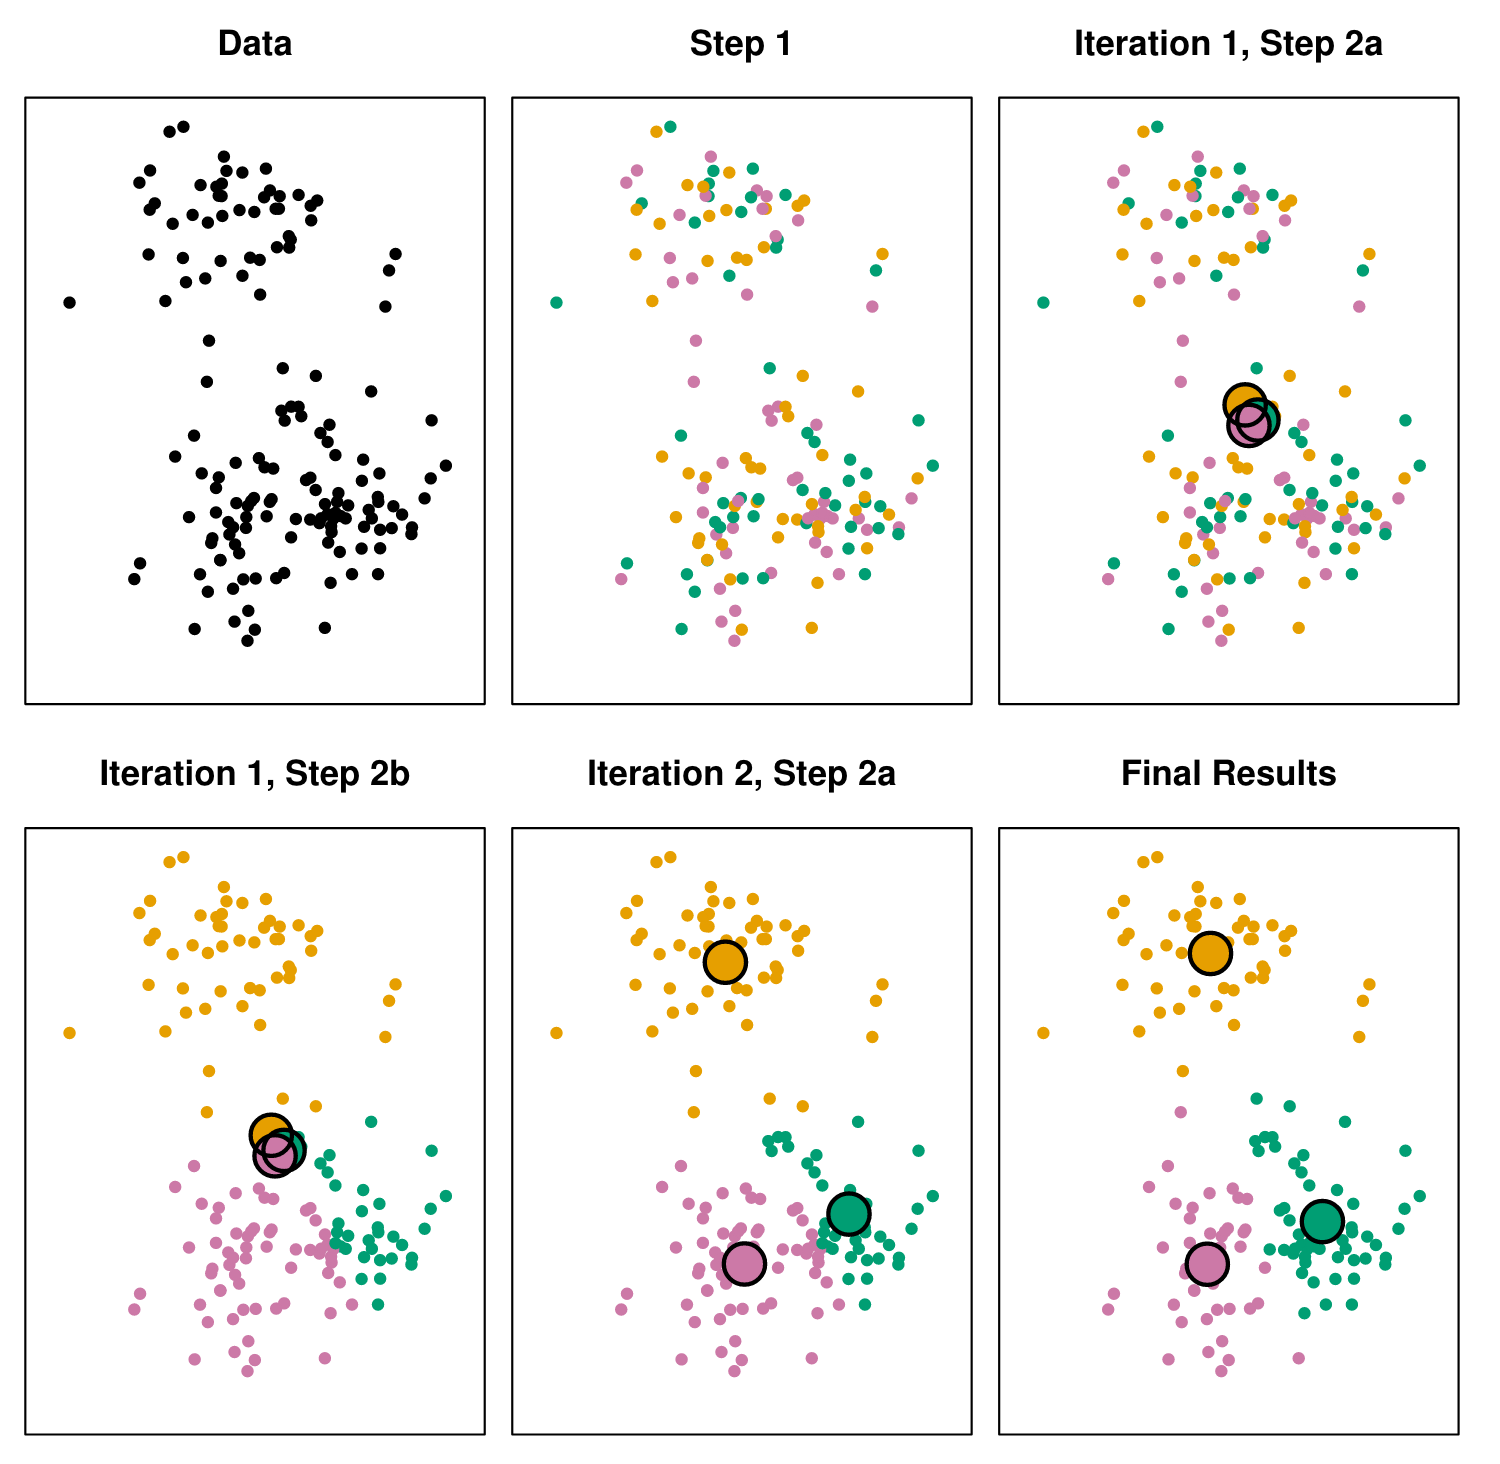
\includegraphics[width=0.6\textwidth]{Images/clustiteration.png}
    \caption[K-Means clustering iterations.]{The progress of the K-means algorithm with $K=3$ \cite{james_introduction_2021}.}
    \label{fig:clustiteration}
\end{figure}
The K-means algorithm progresses through iterative cycles involving two primary actions: (i) assigning data points to clusters and (ii) updating centroids. Given the $K$ centroids, the assignment phase allocates each data point to its nearest centroid, resulting in distinct clusters, where each cluster $C_i$ consists of points closer to its centroid $\bm{\mu}_i$ than to any other centroid. Then, in the update phase, each cluster's centroid is recalculated based on its (updated) member data points. This iterative process of assignment and updating continues until the centroids stabilize. In practical terms, K-means can be considered stable when there's no shift in centroid positions between consecutive iterations. We can adjust the tolerance parameter $\epsilon \geq 0$ for early termination of the algorithm or let the algorithm converge to the local optimum until observations no longer change cluster. In algorithm \ref{alg:kmeans}, there is the pseudo-code of the K-Means clustering algorithm.
\begin{algorithm}
\small
    \caption{K-Means Clustering}
    \label{alg:kmeans}
    \begin{algorithmic}[1]
    \STATE {$t=0$}
    \STATE {Randomly initialize $K$ centroids: $\bm{\mu}_1^t, \bm{\mu}_2^t, \dots, \bm{\mu_k^t} \in \mathbb{R}^p$}
    \REPEAT
    \STATE {$t \leftarrow t + 1$}
    \STATE {$C_i \leftarrow \empty$ for all $i=1,\dots,K$}
    \STATE {//Cluster assignment step}
    \FORALL{$\mathbf{x}_j\in D$}
    \STATE {$i^* \leftarrow \arg \min _i\left\{\left\|\mathbf{x}_j-\boldsymbol{\mu}_i^{t-1}\right\|^2\right\}$}
    \STATE {$C_{i^*} \leftarrow C_{i^*} \cup\left\{\mathbf{x}_j\right\} / / \text { Assign } \mathbf{x}_j \text { to closest centroid }$}
    \ENDFOR
    \STATE {//Centroid update Step}
    \FORALL{$i=1,\dots,K$}
    \STATE{$\boldsymbol{\mu}_i^t \leftarrow \frac{1}{\left|C_i\right|} \sum_{\mathbf{x}_j \in C_i} \mathbf{x}_j$}
    \ENDFOR
    \UNTIL{$\sum_{i=1}^k\left\|\boldsymbol{\mu}_i^t-\boldsymbol{\mu}_i^{t-1}\right\|^2 \leq \epsilon$}
    \end{algorithmic}
\end{algorithm} 
Since the initial guess of the centroids can lead to different labeling of the same observation, the K-means algorithm is typically run several times. In bagging clustering, we run the algorithm multiple times, and the final label is defined by majority voting across the different intermediate clusterizations.
% <<< End of K-means clustering algorithmclassification


% Principal component analysis >>>
\subsection{Principal Component Analysis}
\label{subsec:PCA}
Another unsupervised machine learning technique is the principal component analysis (PCA). This method leverages the information patterns within the dataset to reduce the problem's dimensionality. Principal components (PC) of a set of data in $\mathbb{R}^p$ provide a sequence of best linear approximation to that data of all ranks $q\le p$ \cite{james_introduction_2021, tibshirani_elements_2008}. \emph{Principal component analysis} refers to the process by which principal components are computed. Suppose we have a dataset that represents experience $\mathbf{E}$ of a certain phenomenon, of unlabeled data and each realization $\mathbf{x}_j \in \mathbb{R}^p$ for all $j=1,\dots,n$. Thus, $\mathbf{E} \in \mathbb{R}^{n\times p}$. The first principal component of a set of features $\mathbf{X}_1, \mathbf{X}_2, \dots, \mathbf{X}_p$ is the normalized linear combination of the features
\begin{equation}
    \label{eq:firstPC}
    Z_1=\phi_{11} \mathbf{X}_1+\phi_{21} \mathbf{X}_2+\cdots+\phi_{p1} \mathbf{X}_p
\end{equation}
By normalized, we mean that $\sum_{j=1}^p\phi_{j1}^2=1$. The elements $\phi_{11},\dots,\phi_{p1}$ are the loadings of the first principal component. But how can we find PCs? Suppose we want to find a linear model representing the $i$-th observation. We are trying to find a linear combination such as:
\begin{equation}
    \label{eq:pcaf}
    f(\lambda)=\bm{\mu}+\mathbf{V}_q\bm{\lambda}
\end{equation}
where $\bm{\mu}\in \mathbb{R}^p$ is a location vector, $\mathbf{V}_q$ is a $p\times q$ matrix with $q$ orthogonal unit vectors as columns, and $\bm{\lambda \in \mathbb{R}^q}$ is a vector of $q$ parameters. So, we can fit the model to the data by minimizing the sum of least squared errors:
\begin{equation}
    \label{eq:SSE}
    \min _{\bm{\mu},\left\{\lambda_i\right\}, \mathbf{V}_q} \sum_{j=1}^N\left\|\mathbf{x}_j-\bm{\mu}-\mathbf{V}_q \lambda_j\right\|^2
\end{equation}
We can partially optimize for $\bm{\mu}$ and the $\lambda_j$ to obtain
\begin{equation}
    \hat{\bm{\mu}} = \left(E\left(\mathbf{X}_1\right), E\left(\mathbf{X}_1\right), \dots, E\left(\mathbf{X}_p\right)\right)
\end{equation}
\begin{equation}
    \hat{\lambda}_j = \mathbf{V}_q^{T}(\mathbf{x}_j-\hat{\bm{\mu}})
\end{equation}
This leads to 
\begin{equation}
\label{eq:diocaro}
    \min _{\mathbf{V}_q} \sum_{i=1}^N\left\|\left(\mathbf{x}_j-\hat{\bm{\mu}}\right)-\mathbf{V}_q \mathbf{V}_q^T\left(\mathbf{x}_j-\hat{\bm{\mu}}\right)\right\|^2
\end{equation}
The $q \times q$ matrix $\mathbf{H}_q=\mathbf{V}_q\mathbf{V}_q^T$ is a projection matrix and maps each point $\mathbf{x}_j$ onto it's rank~-~$q$ reconstruction $\mathbf{H}_qx_j$, the orthogonal projection of $x_j$ onto the subspace spanned by the columns of $\mathbf{V}_q$. The solution can be expressed as follows. Stacked the centered observations into rows of an $N\times p$ matrix $\mathbf{E}$, we can construct the singular value decomposition
\begin{equation}
    \label{eq:SVD}
    \mathbf{E}=\mathbf{U}\bm{\Sigma}\mathbf{V}^T
\end{equation}
where $\mathbf{U}$ and $\mathbf{V}$ are unitary matrices and $\bm{\Sigma}$ is a $p \times p$ diagonal matrix, such that $\sigma_{11}\ge \sigma_{22} \ge \dots \ge \sigma_{pp}\ge 0$. This means that $\mathbf{u}_1$ and $\mathbf{v}_1$ correspond to $\sigma_{11}$ and are somehow more important with respect to $\mathbf{u}_2$ and $\mathbf{v}_2$ which are associated to $\sigma_{22}$ in explaining the information in $\mathbf{E}$ and so on and so forth. The columns of $\mathbf{U}$ are the basis vector of the new space, and the columns of $\mathbf{U}\mathbf{D}$ are the principal components. The $\sigma_{ii}$ are also called singular values and are the variance the $i$-th PC explains. Lastly, $\mathbf{v}_i=(\phi_{11} \dots \phi_{p1})$ re the loading vectors of such $i$-th PC.  For each rank $q$, the solution $\mathbf{V}_q$ to Eq. \ref{eq:diocaro}, consist of the first $q$ columns of $\mathbf{V}$. A good method to determine the number $q$ of principal components (PC) is to rely on the scree plot of explained variance. Indeed, the variance explained by each additional PC follows the law of diminishing returns. Therefore, we can decide how many PCs when we observe a significant knee in the graph.

\subsubsection{PCA for Spatial and Temporal Data}
We can also apply PCA to spatial, temporal, or spatiotemporal data. We can also use PCA with images or image streams (videos). Indeed, we can see images as two-dimensional arrays and videos as three-dimensional arrays, in which, along the third dimension, we have time evolution. The most common approach is the \emph{S-mode} PCA, where frame pixels are treated as variables (columns of the dataset) and frames as observations (rows of the dataset). In this way, each frame is unfolded and interpreted as a single dataset entry. By doing so, a video of $J$ frames, each of dimension $M\times N$ can be see as a dataset $\mathbf{X}\in\mathbb{R}^{J\times P}$ where $P=M\times N$. The S-mode captures the correlation of pixels in space to determine how outlying each frame is with respect to the set of considered images. However, the phenomenon's evolution from frame to frame can cause local defects to be hidden. The S-mode PCA approach lacks any spatial localization capability \cite{colosimo_spatially_2018}. Further approaches are the so-called Tensor-based PCA. Multi-linear PCA and the tensor rank-one decomposition are some examples. These methods allow us to pay attention to the temporal effect as in S-mode PCA by not unfolding the image but applying a higher-order PCA. In this sense, the tensor projected onto the low-dimensional space can capture most of the variability of the data, including both spatial and temporal contributions. In the field of quality control, we can use Hotelling's T2, which associates each frame with a synthetic value and makes it possible to identify a shift from the nominal process conditions. Formally, it finds a multi-linear transformation that maps the original tensor space $\mathbb{R}^{M \times N \times J}$ into a tensor subspace $\mathbb{R}^{P_1 \times P_2 \times J}$ with $P_1<M$ and $P_2<N$, where $M$ and $N$ are the dimensions of the video frames. $P_1$ and $P_2$ are the number of PCs retained to capture a given percentage of data variability along the "first mode" (size $M$ ) and "second mode" (size $N$ ) of the original. Lastly, there is also the \emph{T-mode} PCA. This approach interprets the video frames as columns and the pixels as dataset entries. This method captures the temporal auto-correlation of pixel intensity in consecutive frames. In this way, the array $\mathbf{U}\in \mathbb{R}^{M\times N \times J}$ will become the dataset $\mathbf{X}\in \mathbb{R}^{PxJ}$ where $P=M\times N$. The projections of the original image data onto the first retained PCs belong to the image space, and hence, they let a spatial localization of anomalous regions. In this case, however, the spatial S-mode information is completely lost, given that no real distance between pixels is considered. In \citeauthor{colosimo_spatially_2018}, the authors presented an ST-PCA. We will see it in Section \ref{sec:hotspotstateart} as a method to detect HS.

\subsubsection{Handwritten Digits}
This example is  from \citeauthor{tibshirani_elements_2008} (2008).
The authors applied PCA to a dataset containing handwritten digits. Let's consider its application on the digit "3". Authors experimented on a set of 130 3s randomly sampled from a total of 658 total observations. Each image is a \numproduct{16 x 16} gray-scale image. We can see considerable variation in writing styles, character thickness, and orientation (Fig. \ref{fig:3s}). We can unfold images and treat each of them as vectors $\textbf{x}_j \in \mathbb{R}^{256}$, and we can use PCA on the dataset $\mathbf{E}$. In this sense, we are applying an T-mode PCA applied not to the frames of a video but to several images. This technique is also called vectorized PCA (VPCA) because it involves the vectorization operation, also known as unfolding, to transform two-dimensional objects into column vectors. In this way, the projection onto the low-dimensional space will be capable of capturing the most significant spatial variability between the different scripts.
\begin{figure}
    \centering
    \subfloat[\label{fig:3s}]{
        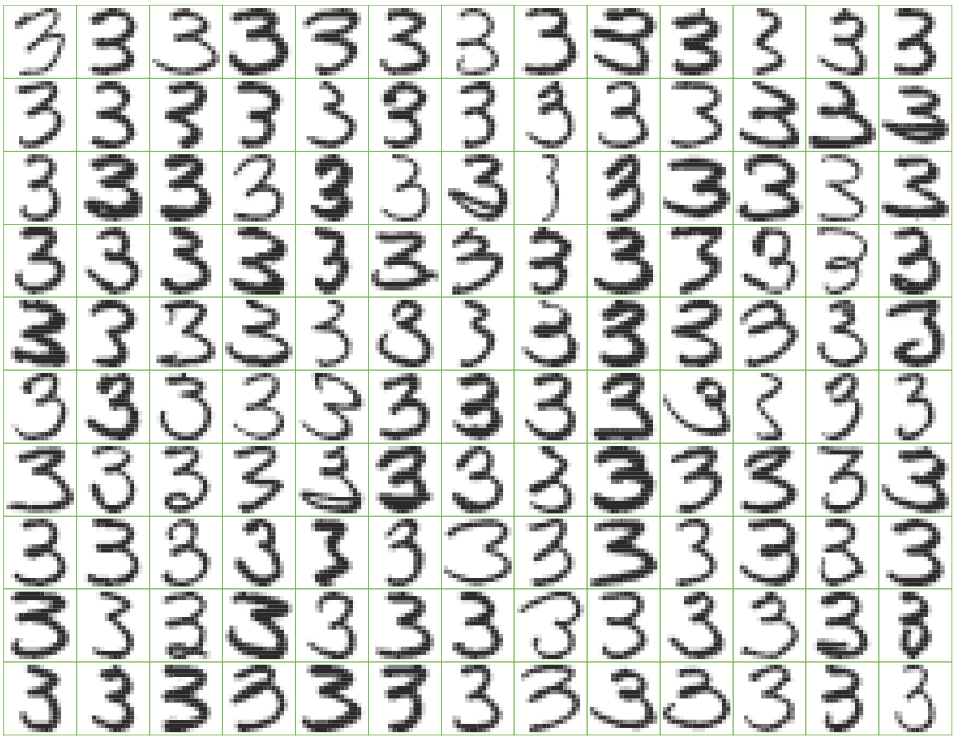
\includegraphics[width = 0.45\textwidth]{Images/1303.png}
    }
    \quad
    \subfloat[\label{fig:principal3}]{
        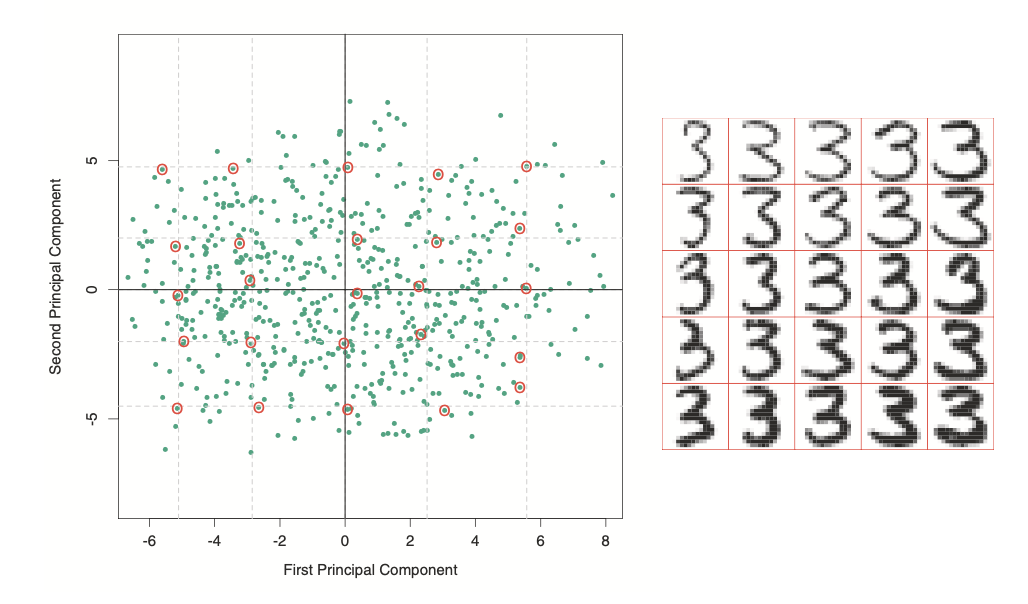
\includegraphics[width = 0.45\textwidth]{Images/pc3.png}
    }
    \caption[Example of PCA of images.]{Example of PCA applaied to images dataset: the random sample of handwritten 3s (a) and the scatterplot of the first two principal components (b) with a superimposed grid in which images match red circles on the scatterplot\cite{tibshirani_elements_2008}.}
\end{figure}
From Fig. \ref{fig:principal3}, we can see that the first PC mainly accounts for the length of the lower tail of the three, while the second PC accounts for character thickness. Then, we can reshape every PC in a matrix and interpret them as images. These images will be the base for the new vectorial space. Using just 50 PCs, we can explain 90\% of the variance of all the 3s, while with 12 PCs, we can account for 63\% of the total variance.


% <<< End of Principal component analysis


%%%%%
%%%%%


% Deep Learning, ANN and CNN >>>
\subsection{Artificial Neural Network and Deep Learnig}
\label{subsec:deepl}
In 1956, there was a summer research project on artificial intelligence at Dartmouth University. A team of professors and an expert from IBM Corporation began to think about the possibility of creating virtual neural networks. These networks would learn and enhance the purpose for which they were designed through a self-improvement process, and they could be based on the mathematical model of the human brain \cite{mccarthy_proposal_1955}. Indeed, the human brain model is especially well-suited for computational purposes. The human brain possesses a massive amount of computing units: the neurons. Approximately \num{e11} neurons in an adult human brain form about 7,000 synaptic connections with other neurons, amounting to nearly \num{e15} total synapses. Moreover, the computational model of the brain is distributed among simple nonlinear units, redundant and fault-tolerant, and capable of performing calculations in parallel \cite{matteo_matteucci_perceptrons_2021}. The mathematical virtual model of a single neuron is called a perceptron, the unitary computational unit of artificial neural networks (ANN). Just like in human neurons, the perceptron has dendrites that "collect" the charge from synapses, and once a certain threshold is exceeded, the accumulated charge is released and sent to other perceptrons. The portion of the schema in Fig. \ref{fig:perceptron} enclosed in the dashed line is called the activation function and is responsible for releasing the perceptron's accumulated charge. There are various activation functions, with some of the most common ones can be seen in Fig. \ref{fig:actfunc}.
\begin{figure}
    \centering
    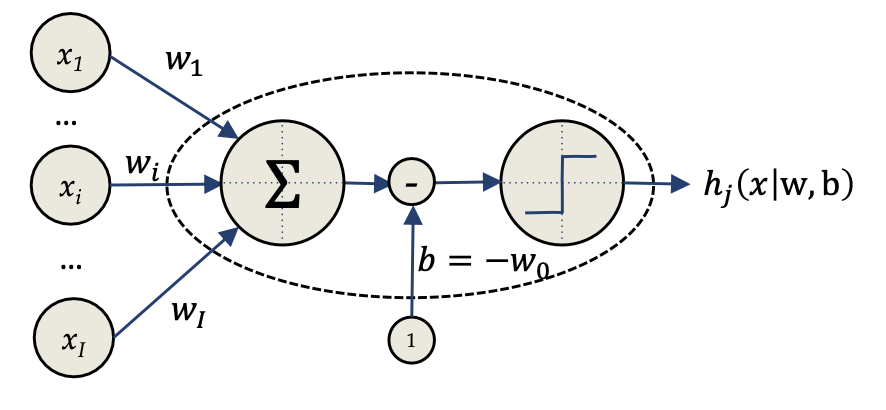
\includegraphics[width=0.6\textwidth]{Images/neurone.png}
    \caption[Perceptron schema]{Perceptron schema \cite{matteo_matteucci_perceptrons_2021}.}
    \label{fig:perceptron}
\end{figure}
Perceptrons can be combined to form networks with a layered architecture. Indeed, every neural network will have an input layer, an output layer, and a varying number of intermediate layers, known as hidden layers. Deep learning is a subfield of artificial intelligence (AI) and machine learning that involves training artificial neural networks on vast amounts of data to perform classification or regression tasks. ANNs can learn from experience $\mathbf{E}$ and understand complex patterns in data. Deep feedforward networks, also called simply feedforward neural networks or multilayer perceptrons (MLPs), are used to approximate some function $f^*$. Let's take as an example a classifier. Given an unknown function $\Lambda_0:E \rightarrow \{1,\dots,L\}$ where $\{1,\dots,L\}$ are label classes, the $f^*$ is the best approximation of the function $\Lambda_0$, defining a mapping $\mathbf{y}=f^*\left(\mathbf{x}, \bm{\theta} \right)$. The ANN learns the value of parameters $\bm{\theta}$ from $\mathbf{E}$, resulting in the best function approximation. These models are called feedforward because information flows through forward all in the network. To understand how neural networks learn from experience $\mathbf{E}$ using the chain rule and the back-propagation mechanism, readers are referred to \citeauthor{goodfellow_deep_2016} (2016).
\begin{figure}
    \centering
    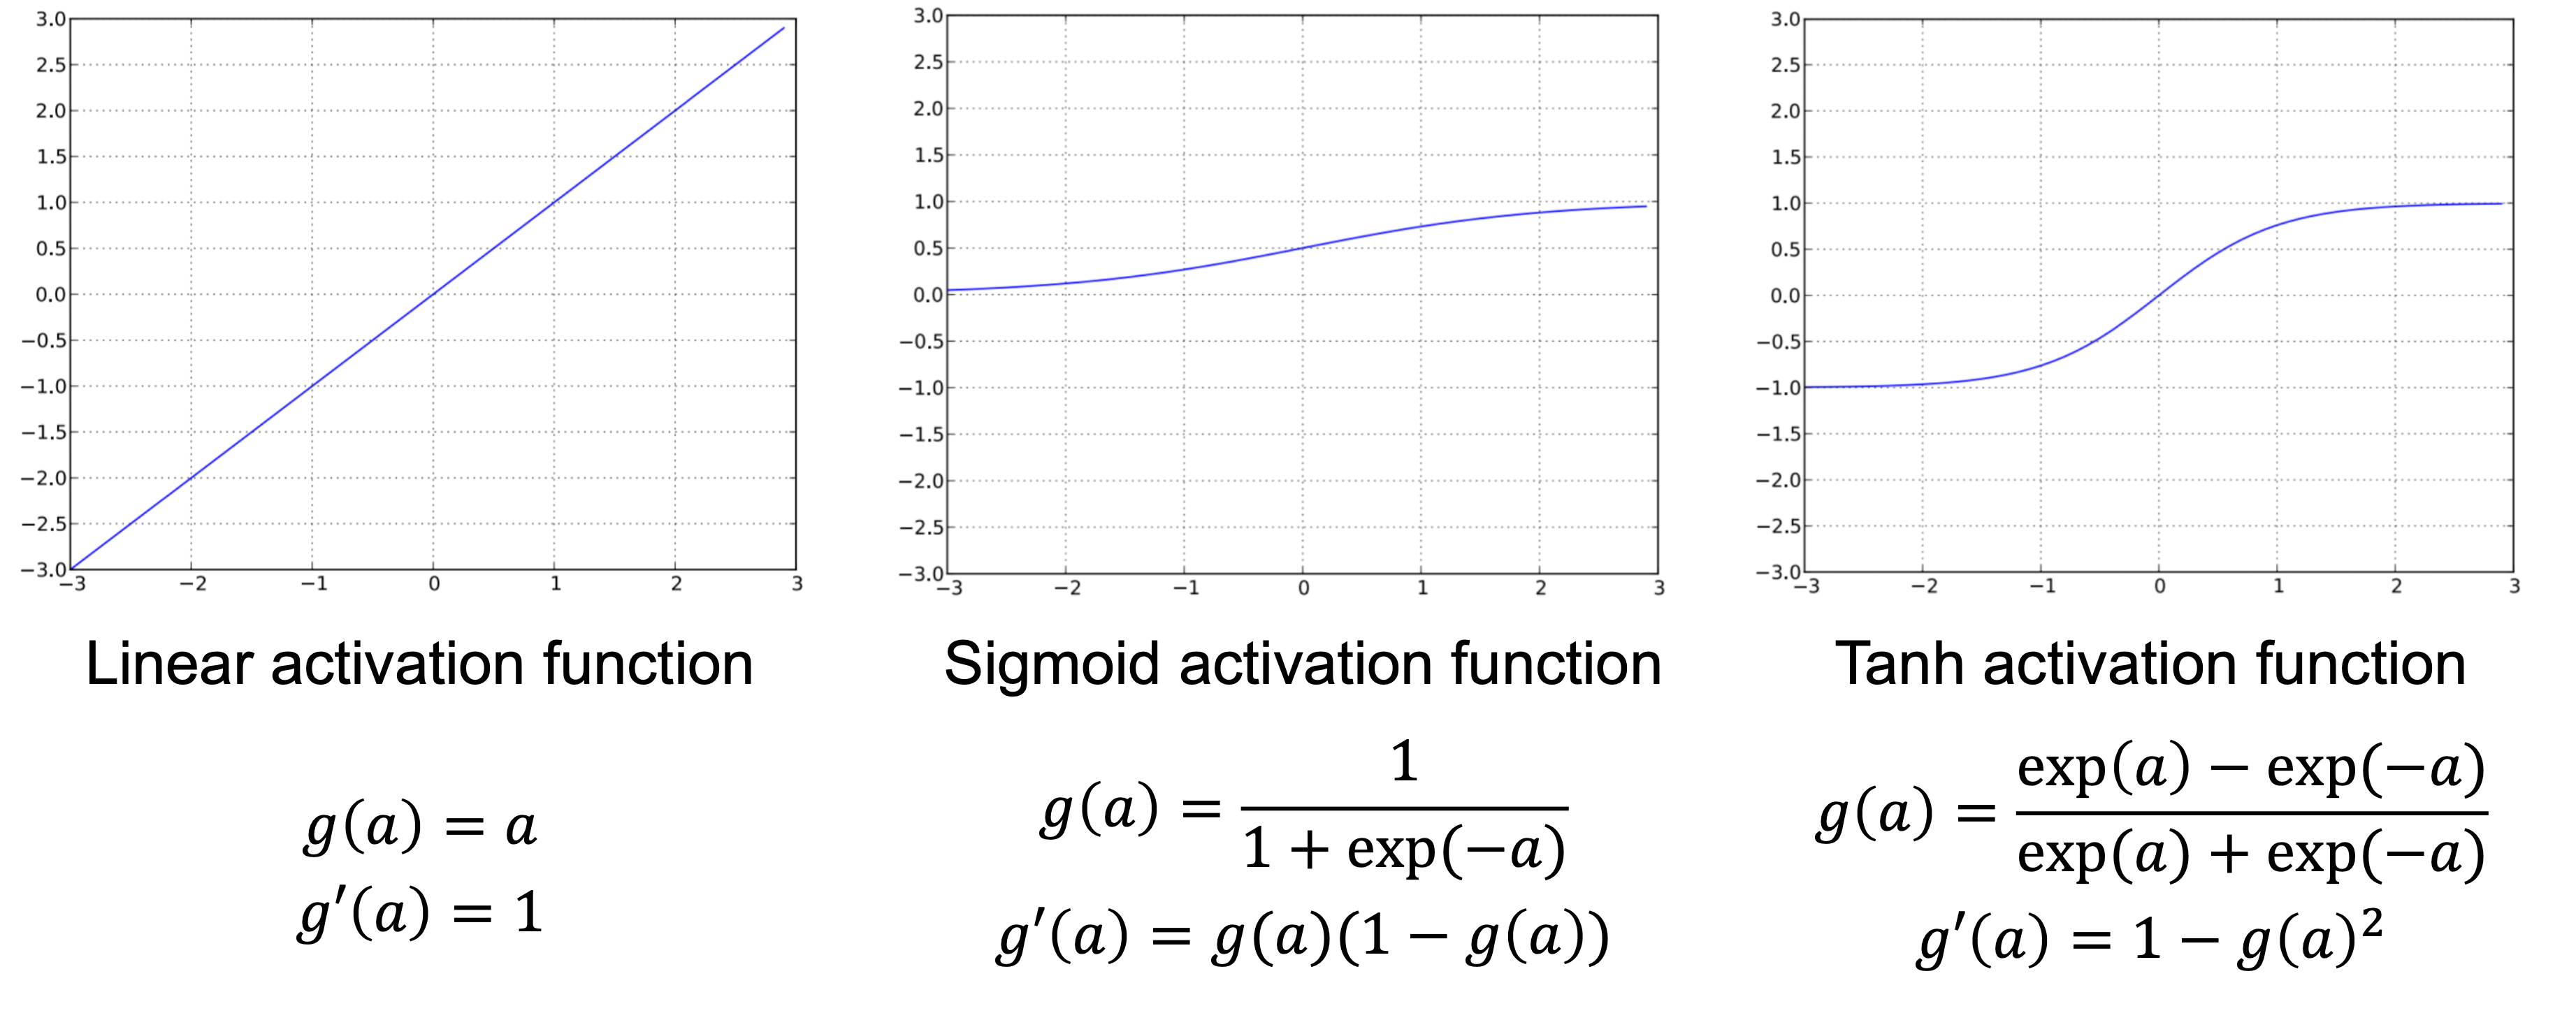
\includegraphics[width=0.8\textwidth]{Images/activationfunction.png}
    \caption[Activation functions.]{Some examples of activation functions with relatives analytical forms \cite{matteo_matteucci_perceptrons_2021}.}
    \label{fig:actfunc}
\end{figure}
Let's examine examples of how networks can address classic machine learning problems such as regression and classification. A best practice is to use tanh or sigmoid as hidden layers activation functions. Indeed, the main difference is the activation function of the output layer: 
\begin{itemize}
    \item \textbf{Regression:} since the output of a regression problem spans all $\mathbb{R}$, the activation function of the output layer will be a linear activation function;
    \item \textbf{Binary Classification:} in binary classification, the output domain is $\Omega=\{0, 1\}$. Thus, the necessary activation function for the output layer is the sigmoid activation function. The value of the function can be interpreted as class posterior probability;
    \item \textbf{Multi-class Classification:} when dealing with multiple classes ($K$), we need to use as many neurons as classes, and each output neuron will use a softmax unit. The unique feature of this activation function is that the sum of the outputs from the $K$ output neurons is equal to 1. Thus, the $k$-th output can be viewed as the probability that the input belongs to the $k$-th class.
\end{itemize}
Another typical application of neural networks is as classification algorithms for images in computer vision. However, images cannot be used directly as input since they carry too much information. We need some intermediate steps to extract useful information and reduce the problem's dimensionality by computing a feature array that summarizes the initial image's information \cite{giacomo_boracchi_convolutional_2021}. The feature array for the input layer of the classification algorithm will have a dimension of $d\ll r_1 \times c_1$ where $r_1$ and $c_1$ are the rows and the columns of the matrix representation of the image. Recall that an image can be represented as a three-dimensional matrix: the first two dimensions are pixel indexes, and the third identifies the pixel's color based on the color profile used. Take, for instance, the image in figure \ref{fig:cazzle}. The image has a width of 472 pixels a height of 376 pixels, and uses an RGB color profile. This means that three values are needed to identify the color of each pixel uniquely: the first for red, the second for green, and the third for blue. This means that we would require \numproduct{472 x 376 x 3} input neurons, one for each value of each color of each pixel of the image (more than 500,000 neurons). Feature extraction algorithms can be categorized as hand-crafted or data-driven features. With hand-crafted algorithms, we can leverage prior knowledge of the phenomenon, and features are interpretable, allowing us to exploit them even with limited data. However, this approach demands significantly more time and design/programming efforts. Moreover, it is very domain-specific and isn't so much "portable". On the other hand, data-driven feature extraction algorithms are less interpretable but offer a more robust mathematical foundation. Convolutional Neural Networks (CNNs) are neural networks that can be used for data-driven feature extraction. Given the matrix representation of the image discussed earlier, while in ANN, we talked about layers, in CNNs, we will have volumes. As the depth of such volumes increases, the height and width of the volume decreases. CNNs enable us to perform some fundamental operations essential for accurate feature extraction.
\paragraph{Convolution.} Convolutional layers "mix" all the input components. Convolution is an operation that allows us to combine all the input values from a specific region into a linear combination. Specifically, the convolution is described by the following equation:
\begin{equation}
    \label{eq:convolution}
    y_j=\sum_iw_{ij}x_i+b_j
\end{equation}
The linear combination operation is also referred to as filtering, and the parameters of this combination are called filters. The same filter is used as a sliding window through the whole spatial extent of the input images. In Fig. \ref{fig:convmatrice}, a typical convolution operation is graphically represented.
\begin{figure}
    \centering
    \subfloat[\label{fig:cazzle}]{
    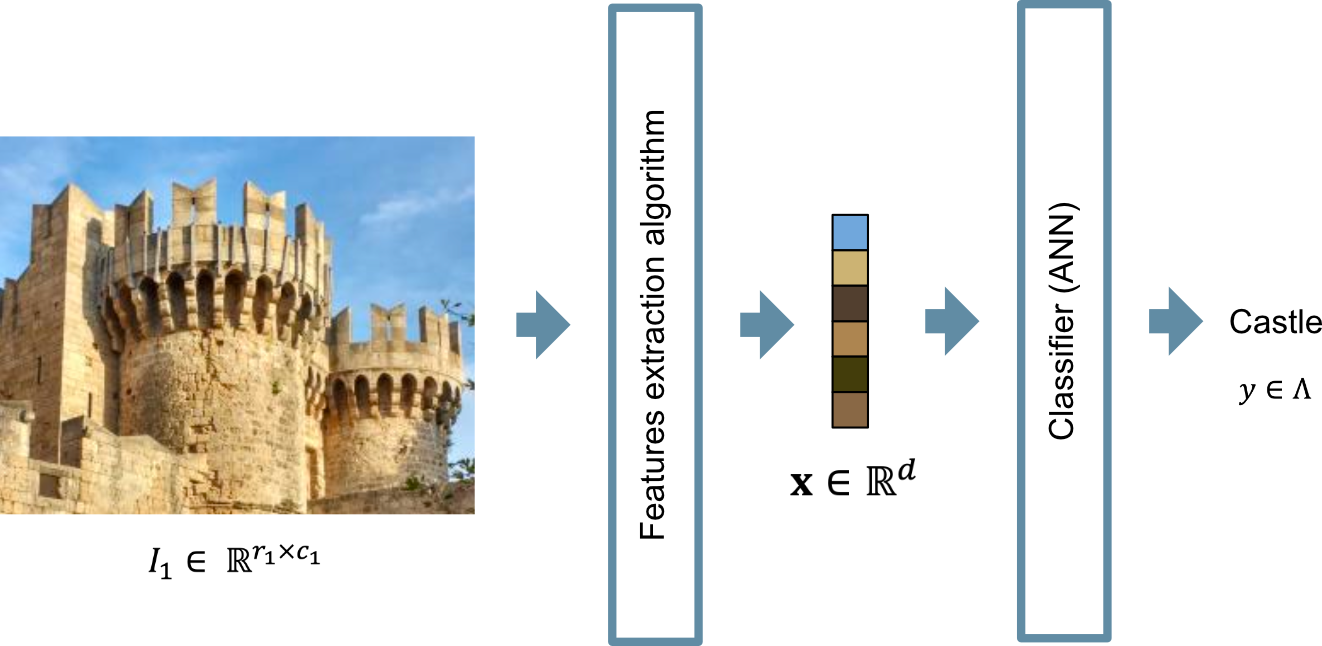
\includegraphics[width=0.7\textwidth]{Images/featureextraction.png}
    }
    \qquad
    \subfloat[\label{fig:convmatrice}]{
    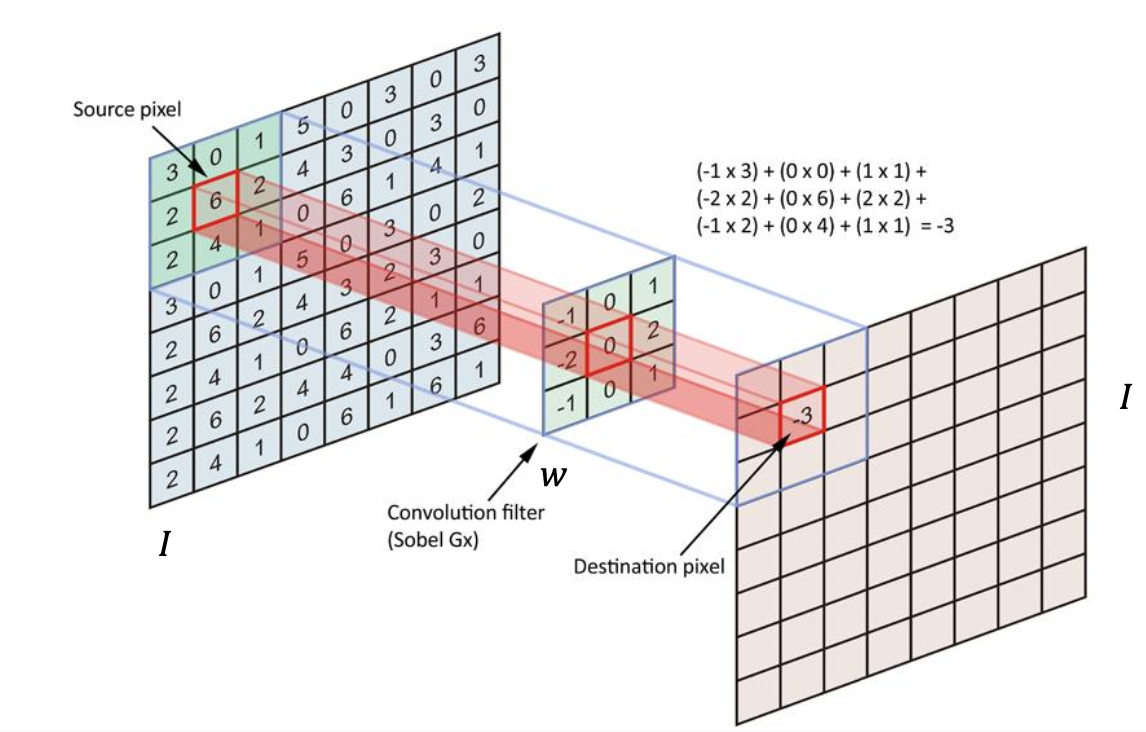
\includegraphics[width=0.5\textwidth]{Images/convolution.png}}
    \caption[Convolution operation.]{Feature extraction operation (a) adapted from \cite{giacomo_boracchi_convolutional_2021}, and convolution operation graphically represented (b)\cite{giacomo_boracchi_convolutional_2021}.}
\end{figure}
In practice, the convolution operation can be viewed as a two-dimensional window that slides across the entire image, producing an output that is a linear combination of the matrix values and their corresponding values.
\paragraph{Pooling layers.} Pooling layers reduce the spatial size of the input volume. Using the logic of a sliding window that traverses the image, a specific function is applied, often the maximum, to spatially resize the input.
\begin{figure}
    \centering
    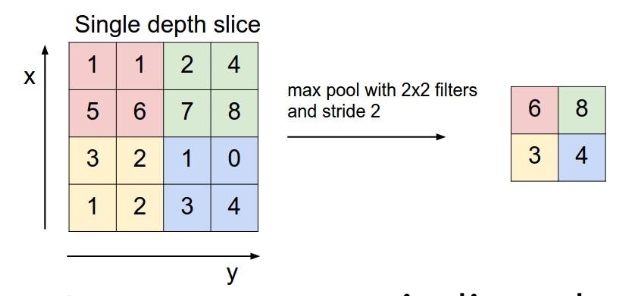
\includegraphics[width=0.5\textwidth]{Images/pooling.png}
    \caption[Pooling layer.]{Example of pooling layer that performs a max operation \cite{giacomo_boracchi_convolutional_2021}.}
    \label{fig:poolingmax}
\end{figure}
The stride parameter specifies how many elements the window shifts at once. In the figure, the window will move by two pixels simultaneously on the y-axis.
\paragraph{Activation layers.} Activation layers are used to introduce non-linearities in the network; otherwise, CNN might be equivalent to a simple linear classifier. In practice, they are layers of neurons characterized by activation functions that introduce non-linearity into the levels, just as in ANNs. We have yet to discuss two commonly used functions in these layers: the RELU (rectified linear units) and LEAKY RELU activation. The former is described as
\begin{equation}
    \label{eq:RELU}
    T(x)=\left\{\begin{array}{rr}
    x, & \text { if } x \geq 0 \\
    0, & \text { if } x<0
\end{array}\right.
\end{equation}
Whereas LEAKY RELU is similar to RELU but incorporates a slight slope for negative values, preventing neurons from dying off and becoming unresponsive after several layers. For a deeper understanding of this topic, one can refer to the vanishing gradient problem as discussed by Goodfellow.
\begin{equation}
    \label{eq:LEAKYRELU}
    T(x)=\left\{\begin{array}{rr}
    x, & \text { if } x \geq 0 \\
    k\cdot x, & \text { if } x<0
\end{array}\right.
\end{equation}
where $k$ is usually in the order of $10^{-2}$.
The convolution output will be a dense feature layer, which implies that this layer can serve as input for an ANN, which will have as many output neurons as classes in the original domain. Fig. \ref{fig:typicalcnn} shows an example of how a general CNN works.
\begin{figure}
    \centering
    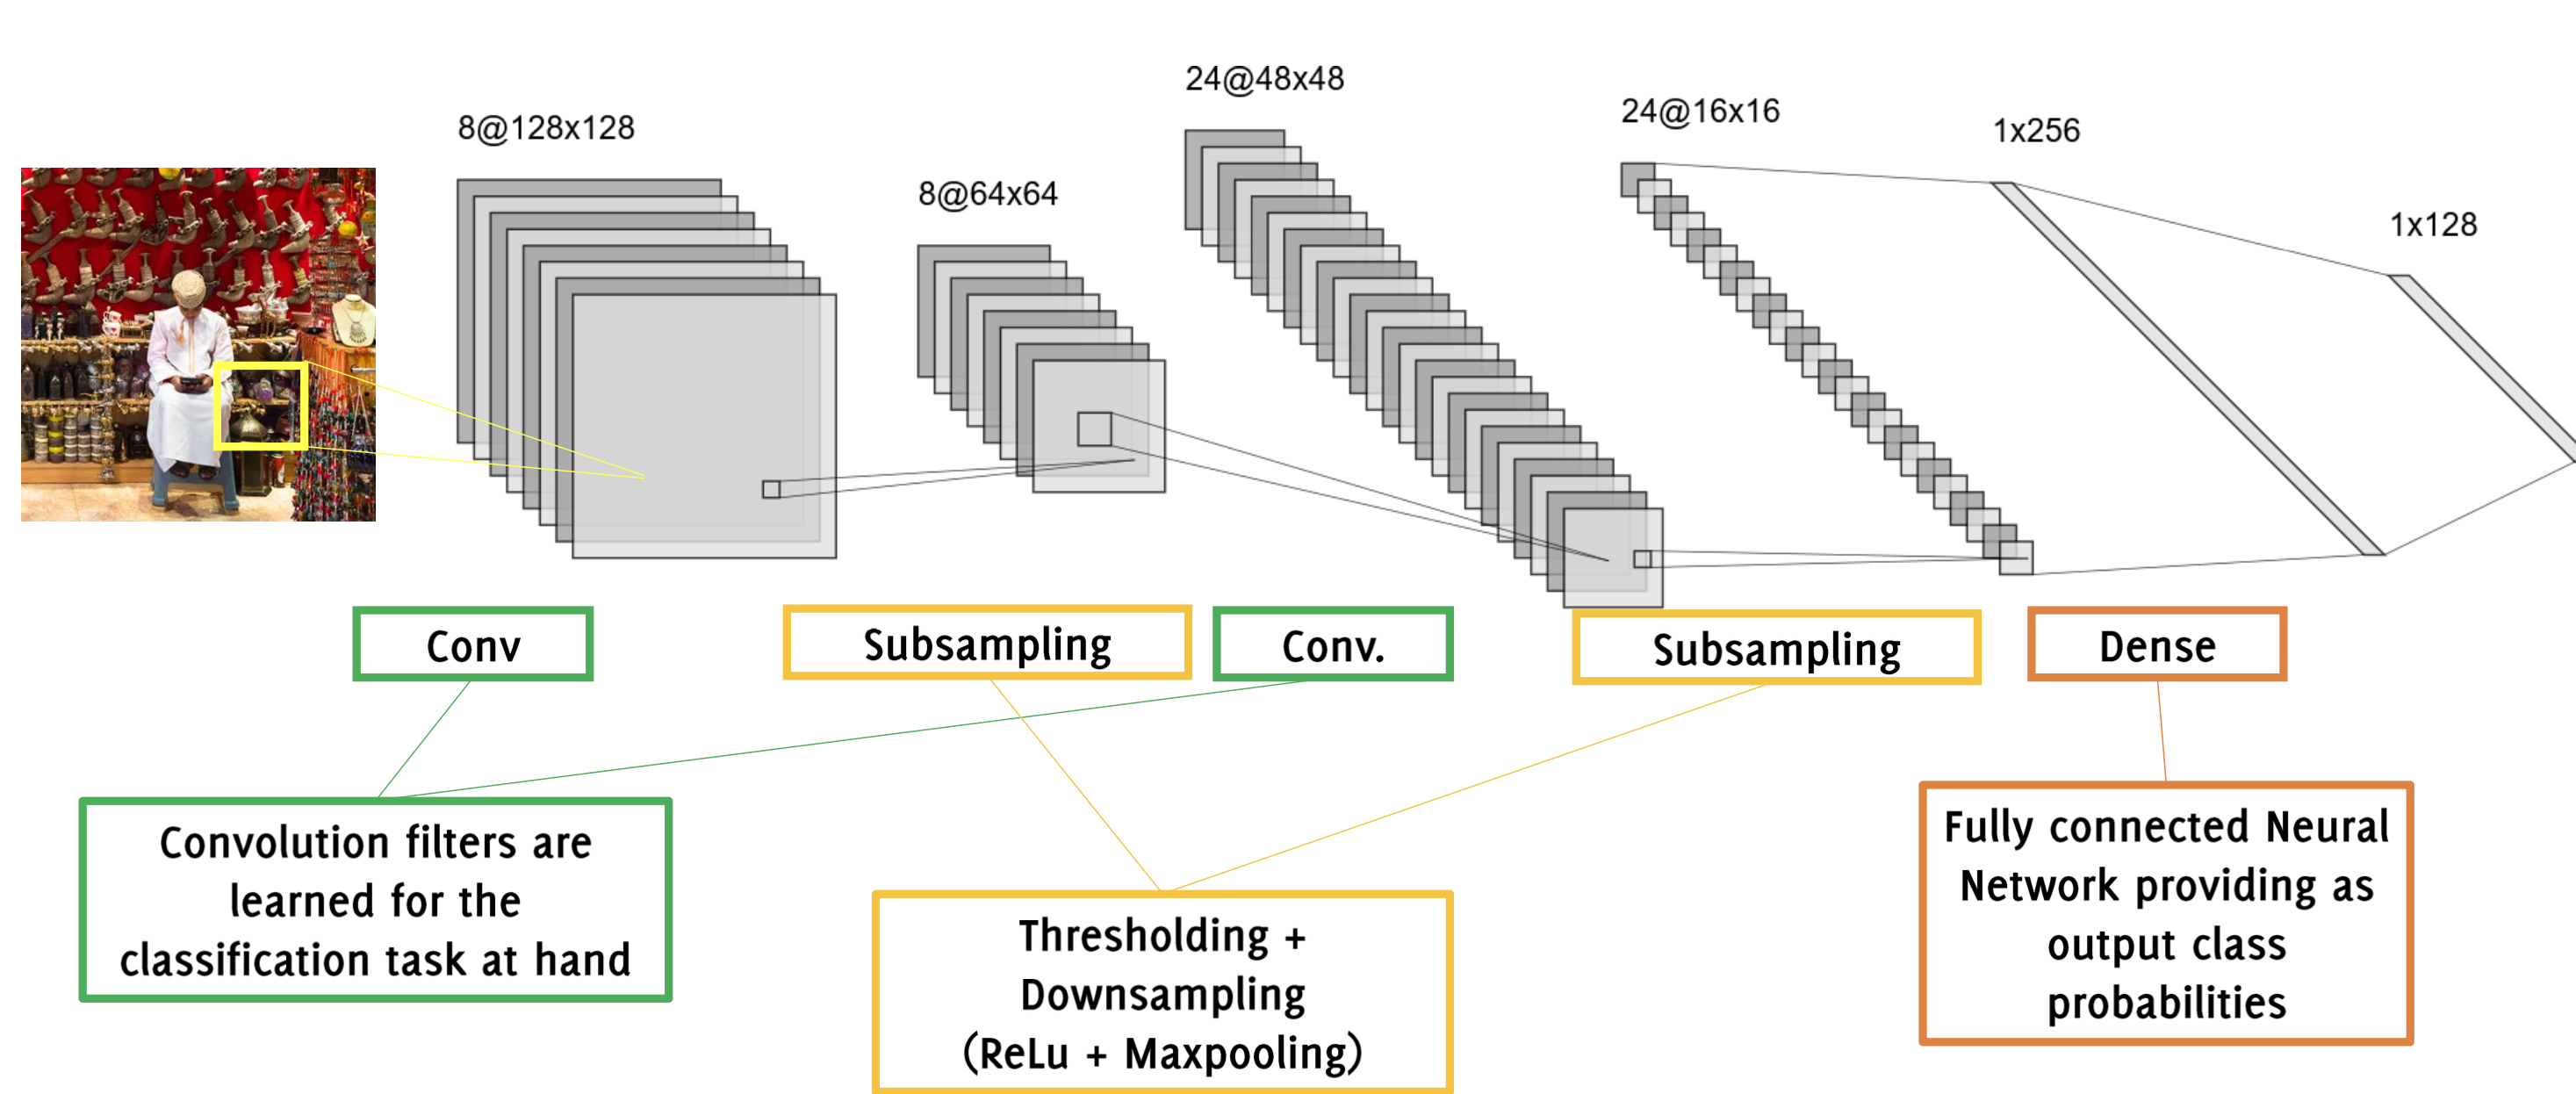
\includegraphics[width=0.8\textwidth]{Images/CNNtypical.png}
    \caption[CNN general structure.]{Graphical representation of a tipical CNN used for image classification \cite{giacomo_boracchi_convolutional_2021}.}
    \label{fig:typicalcnn}
\end{figure}
% End of Deep learning, ANN and CNN


% Deep Belief Network >>>
\subsection{Deep Belief Network}
\label{subsec:dbn}

\begin{figure}
    \centering
    \subfloat[\label{fig:l1}]{
    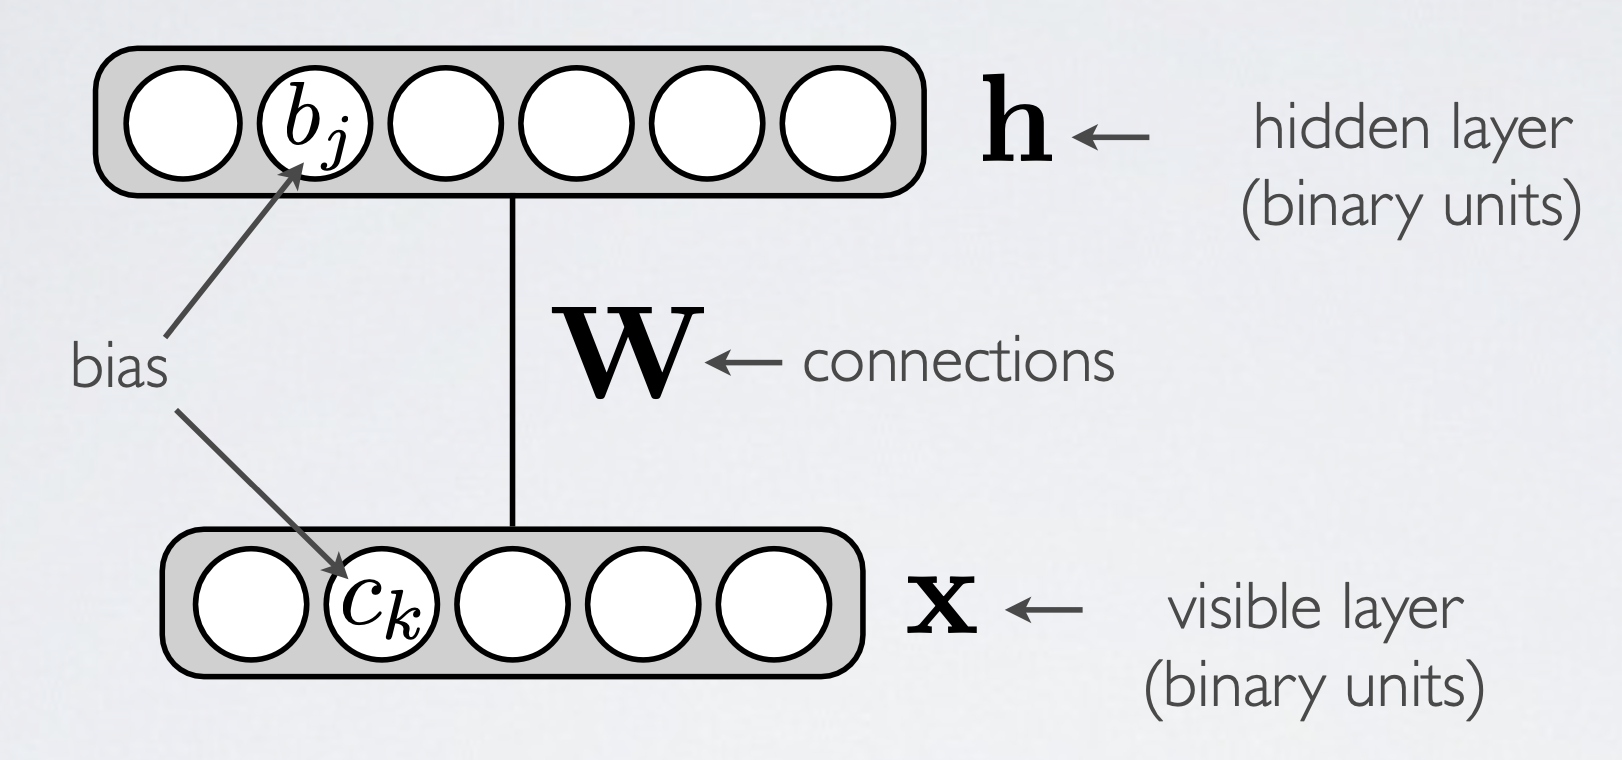
\includegraphics[width=0.4\textwidth]{Images/RBM.png}
    }
    \qquad
    \subfloat[\label{fig:l2}]{
    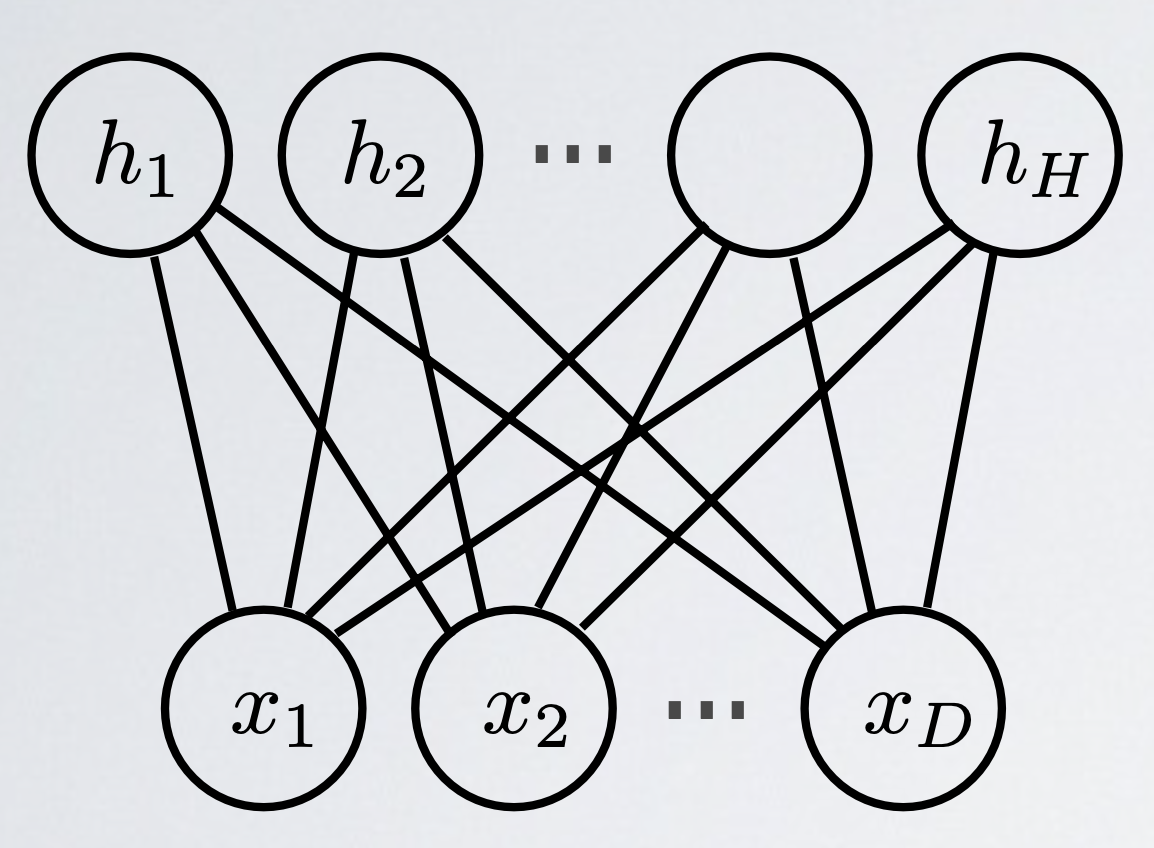
\includegraphics[width=0.3\textwidth]{Images/markovRBM.png}
    }
    \caption[RBM structure.]{Graphical representation of a Restricted Boltzmann Machine (a) and scalar representation of a RBM (b) \cite{hugo_larochelle_neural_2013}.}
\end{figure}
Before explaining what deep belief networks (DBNs) are, it is necessary to explain what Restricted Boltzmann Machines (RBMs) are. RBM can be regarded as a neural network for unsupervised machine learning. This means that they can autonomously extract meaningful features from the data. Mathematically, RBMs are networks made up of symmetrically coupled stochastic binary units. They are determined by a set of visible units $x_k\in[0,1]$, a set of hidden units $x_j\in[0,1]$, and connections between visible and hidden neurons. The RBms will define a distribution over $\mathbf{x}$ involving some latent stochastic variable corresponding to hidden units. Fig. \ref{fig:l1} shows a graphical representation of an RBM. The RBMs are characterized by the presence of an energy function described as
\begin{equation}
\begin{aligned}
E(\mathbf{x}, \mathbf{h}) & =-\mathbf{h}^{\top} \mathbf{W} \mathbf{x}-\mathbf{c}^{\top} \mathbf{x}-\mathbf{b}^{\top} \mathbf{h} \\
& =-\sum_j \sum_k W_{j, k} h_j x_k-\sum_k c_k x_k-\sum_j b_j h_j
\end{aligned}
\end{equation}
In a physical system, the distribution of a particular configuration of a variable of interest can be calculated as 
\begin{equation}
p(\mathbf{x}, \mathbf{h})=\exp (-E(\mathbf{x}, \mathbf{h})) / Z
\end{equation}
and $Z$ is a normalizing factor and is computed as 
\begin{equation}
Z=\sum_{\mathbf{v}, \mathbf{h}} e^{-E(\mathbf{v}, \mathbf{h})}
\end{equation}
The variable set $\theta=(\mathbf{w}, \mathbf{a}, \mathbf{b})$ is parameters to determine the RBM model, and the target of RBM training is to find the optimum $\theta^*$ that represents the training samples.
Suppose the bias $c_k$ is negative and the respective visible neuron $x_k$ equals one. In that case, the energy function will increase, and consequently, the probability of the visible neuron being equal to one will decrease. The network will attribute the zero state to neuron $x_k$. The opposite is also valid; the same applies to the bias $b_j$. The connection matrix $\mathbf{W}$, on the other hand, will help to consider the interaction between neurons. Indeed, if we represent the network in vector form as in Fig. \ref{fig:l2}, we can easily rewrite the probability distribution by highlighting the joint and single effects
\begin{equation}
p\left(\mathbf{x},\mathbf{h}\right) = \overbrace{\frac{1}{Z}\prod_j \prod_k \exp\left(W_{j,k}h_jX_k\right)}^\text{pair-wise factors} \quad \overbrace{\prod_j \exp\left(c_kx_k\right) \prod_k \exp\left(b_jh_j\right)}^\text{unitary factors}
\end{equation}
A typical example of RBMs use is in recommendation engines, where they are used as collaborative filters. Each visible neuron tells us whether a user will like a given content given another that he or she has liked. To better understand the potential of these networks, let us take the dataset of handwritten digits from the previous example as an example. Remember that each image is binary with dimensions \numproduct{16 x 16} pixels. After vectorizing the images, we define 256 visible neurons such that there is one neuron for each image pixel. We then move on to the training phase. Once the training phase is complete, we can take all the connections that join a hidden neuron to the visible neurons. We obtain a vector of connections $\mathbf{w} \in \mathbb{R}^256$ that we can rescale into a matrix $16 \times 16$ and interpret as an image. For each hidden neuron, we obtain an image like those in Fig. \ref{fig:minstbrm}. Let us now consider the matrix highlighted in red. Grey values are connections with weights close to zero, white values are positive, and black values are negative. This means that the hidden neuron has detected that the direction of the line indicated by the red arrow is a relevant feature for maximizing the representation capacity of the training dataset.
\begin{figure}
    \centering
    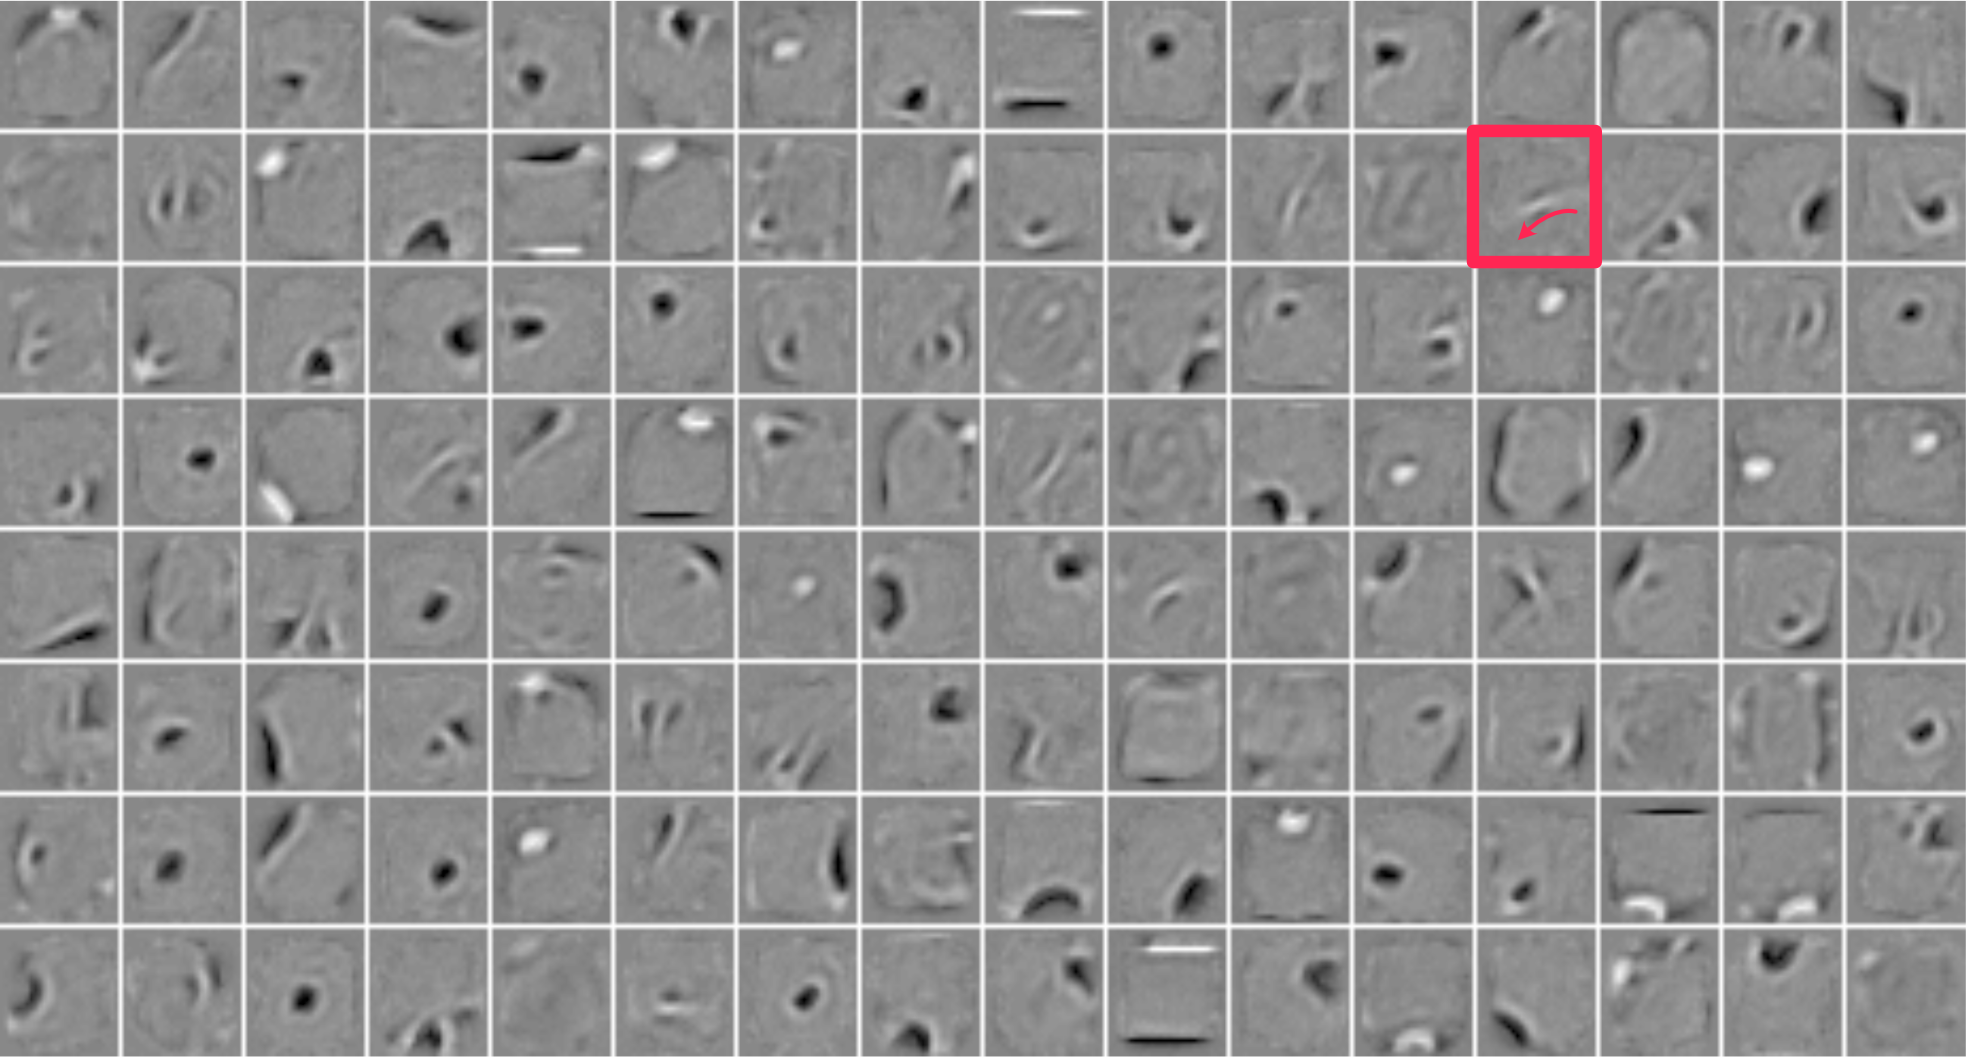
\includegraphics[width=0.7\textwidth]{Images/mnistrbm.png}
    \caption[RBM connection matrixes.]{Example of connections between visible and hidden neurons extracted from the handwritten digits dataset \cite{hugo_larochelle_neural_2013}.}
    \label{fig:minstbrm}
\end{figure}
A Deep Belief Network(DBN) is a powerful generative model that use a deep architecture of multiple stacks of Restricted Boltzmann machines(RBM). In particular, it is a generative model based on directed and undirected connections between nodes. The top 2 layers, in Fig. \ref{fig:dbnhugo}, the $\mathbf{h}^{(3)}$ and $\mathbf{h}^{(2)}$ layers are an RBM, while the other layers are layers of a Bayesian Network. This means that a conditional probability distribution with respect to the previous layer describes them. Indeed, the probabilistic distributions of these layers are
\begin{equation}
\begin{aligned}
p\left(h_j^{(1)}=1 \mid \mathbf{h}^{(2)}\right) & =\operatorname{sigm}\left(\mathbf{b}^{(1)}+\mathbf{W}^{(2)^{\top}} \mathbf{h}^{(2)}\right) \\
p\left(x_i=1 \mid \mathbf{h}^{(1)}\right) & =\operatorname{sigm}\left(\mathbf{b}^{(0)}+\mathbf{W}^{(1)^{\top}} \mathbf{h}^{(1)}\right)
\end{aligned}
\end{equation}
Recall that sigmoid functions $\operatorname{sigm}(z)$ is defined as
\begin{equation}
\operatorname{sigm}(z)=\frac{1}{(1+\exp (-z))}
\end{equation}
Since the distribution is defined by the sigmoid function, these layers are called sigmoid belief networks. The unique feature of DBNs is the ability to learn a hierarchical probabilistic model efficiently due to the level-by-level training that can be repeated several times. During the final phase of DBN training, all parameters found during the first unsupervised training phase are adjusted using a supervised learning technique using initial values obtained from the previous training stage.
\begin{figure}
    \centering
    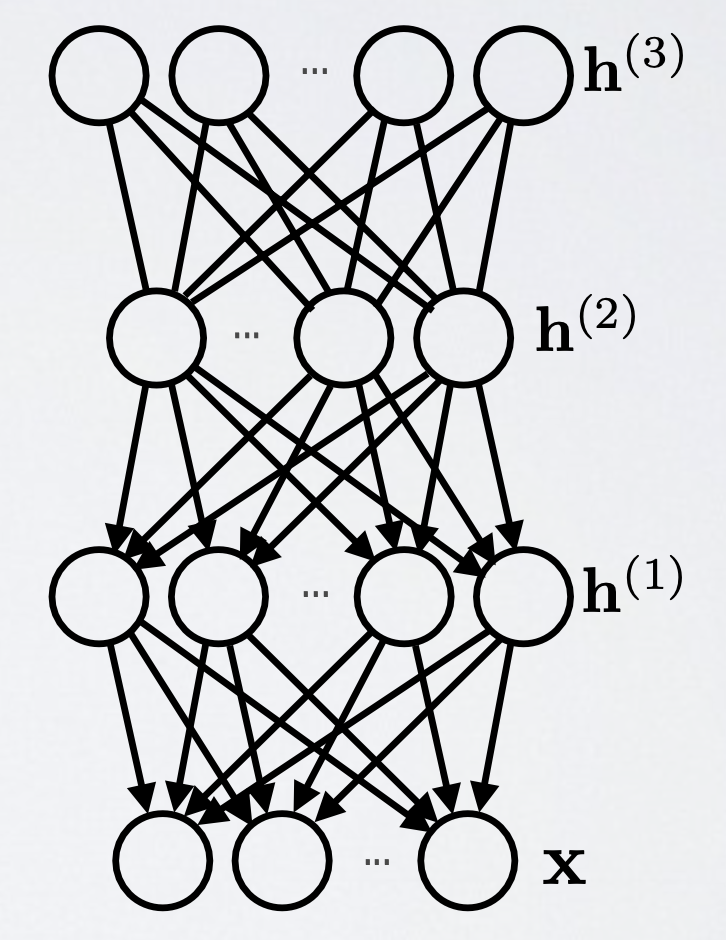
\includegraphics[width=0.25\textwidth]{Images/DBN graphical.png}
    \caption[DBN graphically represented.]{A graphical representation of a deep belief network \cite{hugo_larochelle_neural_2013}.}
    \label{fig:dbnhugo}
\end{figure}
% <<< End of Deep Belief Network

%%%%%
%%%%%

% Hot spot >>>
\section{Hot-Spot Detection Using ML Algorithm}
\label{sec:hotspotstateart}
This section will systematically review the literature on machine learning algorithms used for hot spot detection. The search strategy with the queries used, and the results are explained in detail in Appendix \ref{ap:research}. Table \ref{tab:slr} shows the papers selected for the literature review.
\begin{table}
\centering
\begin{tabular}{llllll}
\hline
\tiny
Author & \tiny
  Year & \tiny
  Process & \tiny
  Sensor & \tiny
  Proposed method & \tiny
  Reference \\ \hline 
  \tiny
\begin{tabular}[c]{@{}l@{}}Bugatti M.,\\ Colosimo B. M.\end{tabular} & \tiny
  2021 &
    \tiny L-PBF & \tiny
  \begin{tabular}[c]{@{}l@{}}High speed camera \\ (CMOS sensor)\end{tabular} &\tiny
  \begin{tabular}[c]{@{}l@{}}k-means FD clustering,\\ SVM, ANN\end{tabular} & \tiny \cite{bugatti_towards_2022}
   \\[0.3cm]
 \tiny \begin{tabular}[c]{@{}l@{}}Colosimo B. M.,\\ Grasso M\end{tabular} & \tiny
  2018 & \tiny
  L-PBF & \tiny
  \begin{tabular}[c]{@{}l@{}}High speed camera \\ (CMOS sensor)\end{tabular} & \tiny
  Weighted PCA & \tiny \cite{colosimo_spatially_2018}
   \\[0.4cm]
\tiny \begin{tabular}[c]{@{}l@{}}Yan H., \\ Grasso M, \\ Paynabar K.,\\ Colosimo B. M.\end{tabular} & \tiny
  2020 & \tiny
  L-PBF & \tiny
  \begin{tabular}[c]{@{}l@{}}High speed camera \\ (CMOS sensor)\end{tabular} & \tiny
  \begin{tabular}[c]{@{}l@{}}Penalized \\ spatio-temporal \\ regression\end{tabular} & \tiny \cite{yan_real-time_2021}
   \\[0.5cm]
\tiny \begin{tabular}[c]{@{}l@{}}Grasso M.,\\ Laguzza V.\\ Semeraro Q.,\\ Colosimo B. M.\end{tabular} &
  \tiny 2017 &
  \tiny L-PBF &
  \tiny \begin{tabular}[c]{@{}l@{}}High speed camera \\ (CMOS sensor)\end{tabular} & \tiny
  K-Means Clustering & \tiny \cite{grasso_-process_2017}
   \\[0.5cm]
\tiny \begin{tabular}[c]{@{}l@{}}Baumgartl H.,\\ Toma J.,\\ Buettner R., \\ Merkel M.\end{tabular} & \tiny
  2020 & \tiny
  L-PBF & \tiny
  Thermographic camera & \tiny
  CNN & \tiny \cite{baumgartl_deep_2020}
   \\[0.6cm]
\tiny \begin{tabular}[c]{@{}l@{}}Mao Y., Lin Hui, \\ Xuan Yu C., Frye R., \\ Beckett D., Anderson K., \\ Jacquemetton L., \\ Carter F., Gao Z., \\ Liao W. , Choudhary A. N., \\ Ehmann K., Agrawal A.\end{tabular} & \tiny
  2022 & \tiny
  L-PBF & \tiny
  Thermographic camera & \tiny
  CNN & \tiny \cite{mao_deep_2023}
   \\[1cm]
\tiny \begin{tabular}[c]{@{}l@{}}Ye D., \\ Soon Hong G., \\ Zhang Y., Zhu K., \\ Ying Hsi Fuh J.\end{tabular} &
  \tiny 2017 &
  \tiny L-PBF &
  \tiny \begin{tabular}[c]{@{}l@{}}Acoustic Sensor \\ (microphone)\end{tabular} &
  \tiny DBN & \tiny \cite{ye_defect_2018}
   \\[0.5cm] \hline
\end{tabular}
\caption{Summary of analyzed papers.}
\label{tab:slr}
\end{table}
Fortunately, many of these papers present methods that have been applied to the same dataset. Thus, we can compare different approaches and see how the different approaches perform on the same data obtained under the same conditions. All the analyzed papers propose approaches to HS detection in L-PBF processes. This is probably because, as mentioned above, collecting data for level 2 and level 3 process signatures is more difficult in EB-PBF processes, mainly due to the fact that external sensors are hard to install. Indeed, in L-PBF processes, it is easier to identify this type of anomaly as a more uniform pixel pitch characterizes the powder bed. Due to the high energy penetration within the metal material in EBM processes, the images show bright areas that interfere with measurement tasks. This causes several pre-processing operations to be required before analysis can take place \cite{grasso_powder_2020}. However, during the snowballing process described in Section \ref{sec:resmetodologies}, I found some examples of HS detection in EBM processes, which did not, however, use ML-based approaches. For example, in \citeauthor{grasso_powder_2020} (2020), the authors were able, using a high spatial resolution camera and a high temporal resolution camera, to calculate a summary index of the image to raise an alarm indicating the presence of a HS. This index exploits the anomalous behavior of the HS of the pixel intensity profiles. The HS presents a profile characterized by a high intensity maintained for a specific time interval and a subsequent slow cooling transitory. The synthetic index was computed as 
\begin{equation}
    \label{eq:sinteticgrassohs}
    S_I(x, y)=\sum_{t=0}^T \mathcal{I}\left( I_t(x, y) > k_1 \text{and} \Delta I(x, y<k_2 \right)
\end{equation}
where $\mathcal{I}(\cdot)$ is the indicator function, $I_t(x, y)$ is the pixel intensity of the $(x, y)$-th pixel in the $t$-th frame, $\Delta I(x, y)$ is the difference of $(x, y)$-th pixel intensities in the $t$-th and $(t-1)$-th frames and $k_1$ and $k_2$ are constants to be defined during a calibration phase. The authors also proposed a method for choosing $k_1$ and $k_2$ values, and for the data collected during the study, these values were set to 90\% and 10\%, respectively. The estimate of $S_I(x, y)$ can be iteratively updated as new video frames are acquired. The proposed algorithm is worthwhile for defect detection only and does not lead to any additional conclusion from temporal and spatial analysis.

We can now move on to the papers analyzed during the research of this thesis topic. In order to give as structured an approach as possible, papers are classified by the proposed method. This section follows the diagram in Fig. \ref{fig:SLRdiagramma}. This section will first illustrate machine learning methods and then deep learning approaches.
\begin{figure}
    \centering
    \subfloat[\label{fig:SLRdiagramma}]{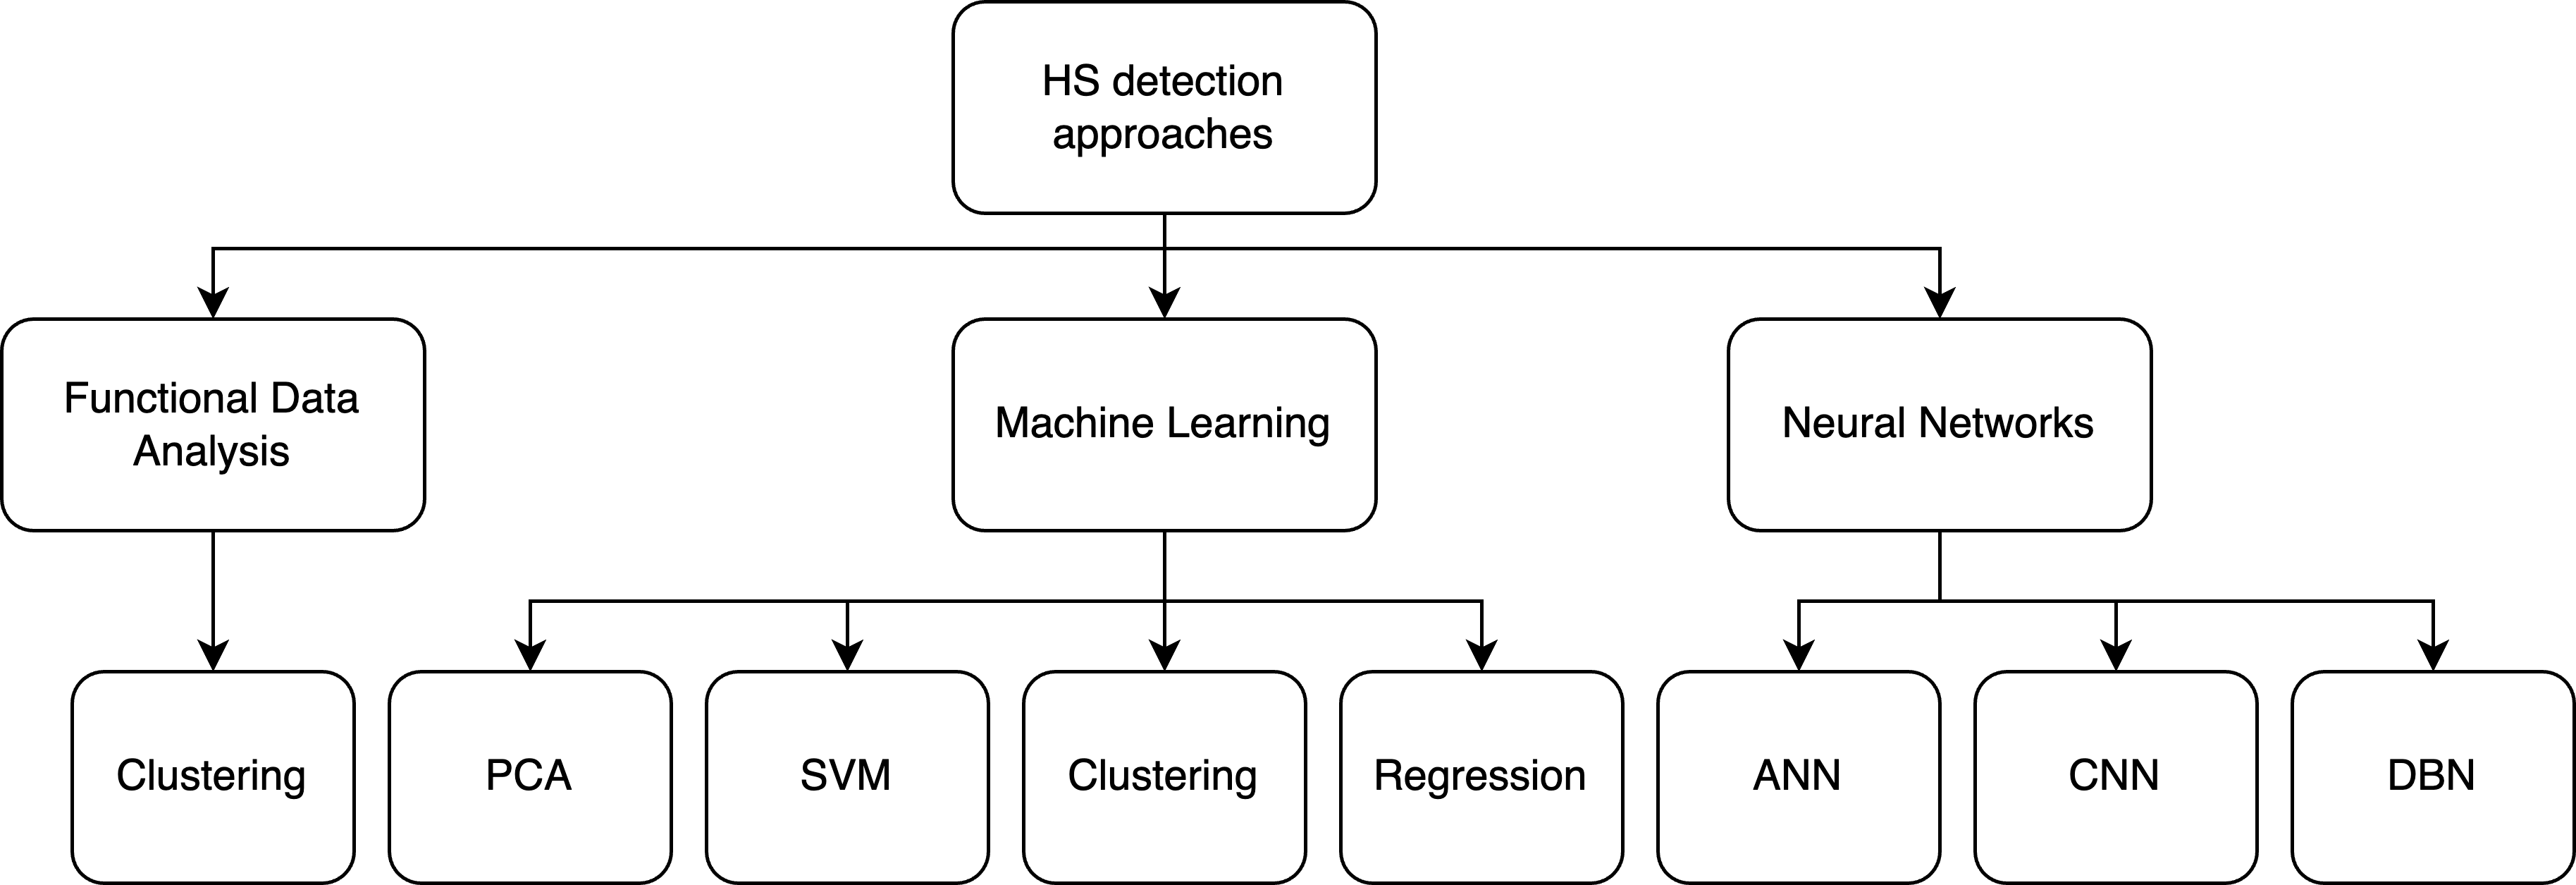
\includegraphics[scale=0.12]{Images/SLR diagram.png}}
    \qquad
    \subfloat[\label{fig:hsgrassoebm}]{
    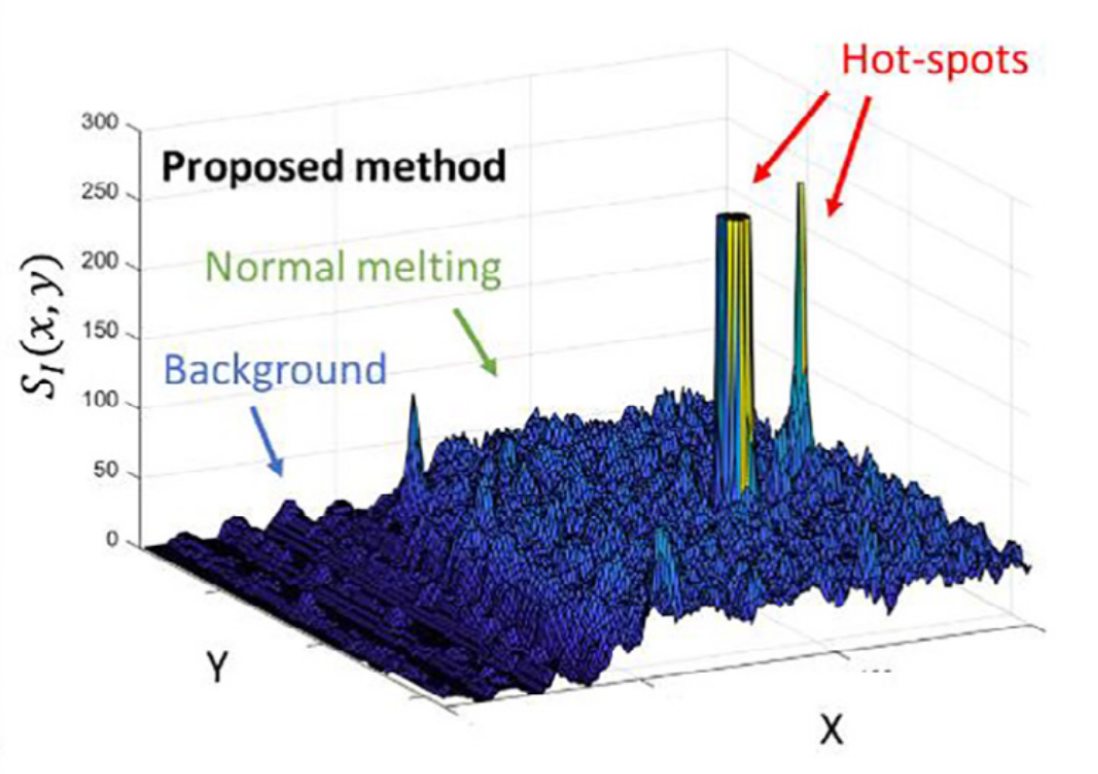
\includegraphics[width=0.4\textwidth]{Images/ebmgrassohs.png}}
    \qquad
    \subfloat[\label{fig:HSframes}]{
    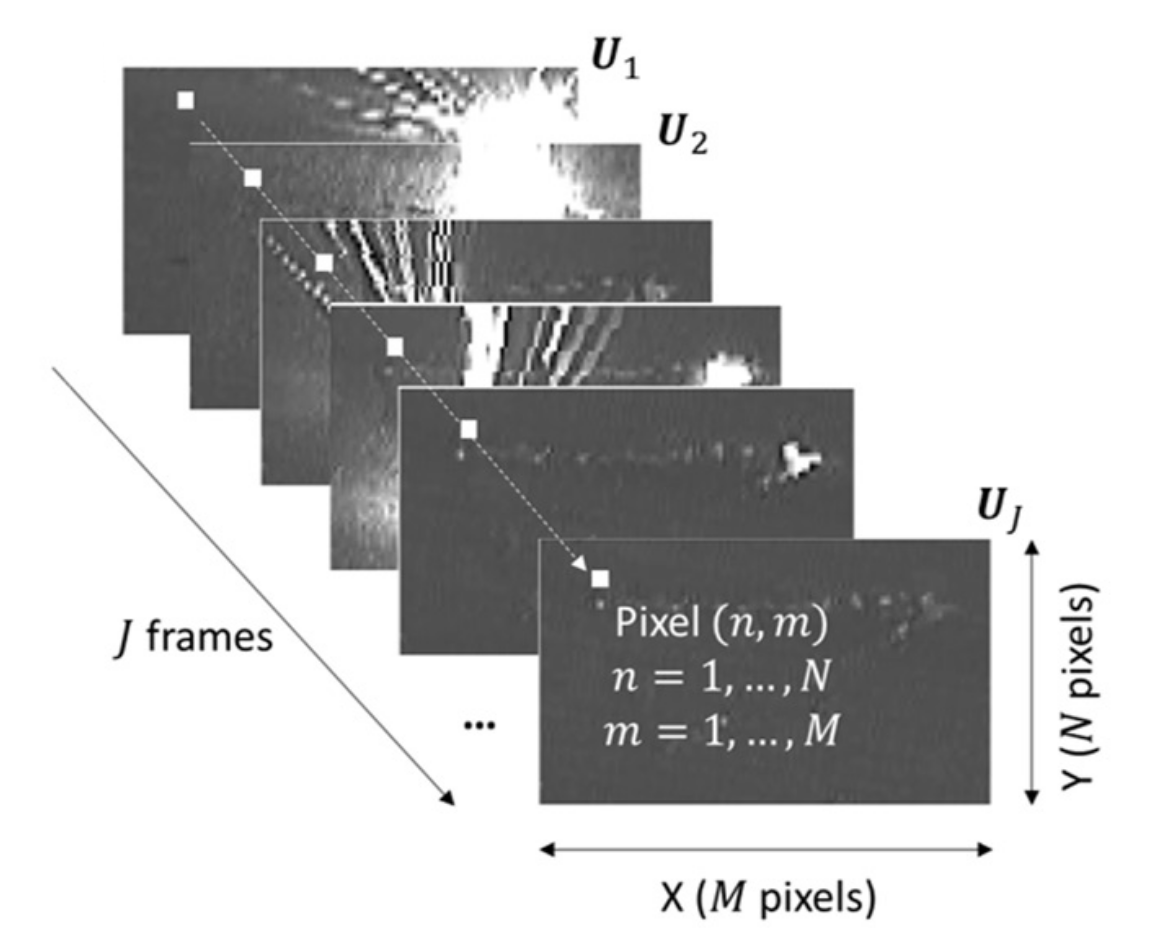
\includegraphics[width=0.4\textwidth]{Images/framesPCAHS.png}
    }
    \caption[Hot spots detection.]{Breakdown of analyzed papers according to the approach used (a), hot-spot detection in EBM with synthetic index (b) \cite{grasso_powder_2020}, frames acquired for spatially weighted PCA (c) \cite{colosimo_spatially_2018}}
\end{figure}

\paragraph{PCA and Hotelling's $T^2$ distance.} In \citeauthor{grasso_-process_2017} (2017), authors proposed a method to perform in-process monitoring of an SLM process using image analysis. With this method, we are able to identify the spatial localization of local defects due to overheating phenomena. The proposed approach relies on PCA and Hotelling's $T^2$ distance in conjunction with an automated defect detection technique based on k-means clustering. Unlike some approaches we will see later, the peculiarity of this method is that it does not require any a priori ad-hoc segmentation, avoiding pre-processing operations such as thresholding. The authors printed the complex shape in Fig. \ref{fig:complexhs} measuring \numproduct{50x50x50} \unit{\milli\metre} using AISI 316 L powder via SLS. During the process, they acquired a video using an OlympusTM I-speed 3 camera (CMOS sensor) placed outside the build chamber viewport with an acquisition rate of 300fps. The acquired stream of gray-scale video images (Fig. \ref{fig:HSframes}) can be described in terms of a 3-dimensional array, $U=\left\{\boldsymbol{U}_1, \boldsymbol{U}_2, \ldots, \boldsymbol{U}_J\right\} \in \mathbb{R}^{J \times M \times N}$, where $M \times N$ is the size (in pixels) of each frame and $J$ is the total number of acquired frames over a time period of duration $T=J / f$, being $f$ the sampling frequency. $\boldsymbol{U}_j \in \mathbb{R}^{M \times N}$ is the $j$-th image, $j=1, \ldots, J$, and $\boldsymbol{u}_{m, n}=\left\{u_1(m,n), u_2(m, n), \ldots, u_J(m,n)\right\}$ is the intensity profile of the pixel at location $(m, n)$ over the $J$ acquired frames, with $n=1, \ldots, N$ and $m=1, \ldots, M$. The pixel intensity $u_j(m,n)$ ranges from 0 to 255, where 0 is black and 255 is white. Subsequently, individual frames were extracted from the video and vectorized in order to obtain a T-PCA. Thus, the three-dimensional array $\mathcal{U} \in \mathbb{R}^{J \times M \times N}$ is transformed into a matrix $\mathbf{X} \in \mathbb{R}^{p \times J}$, where $p=M \times N$. Each row of the matrix consists of a pixel intensity profile, i.e., the $1 \times J$ vector $\boldsymbol{u}(m, n)=\left[u_1(m, n), \ldots, u_J(m, n)\right]^{\mathrm{T}}$. The VPCA generates PCs that associate a weight to each frame. Hence, each PC is a $1 \times J$ vector that weights each time-location of pixel intensity profiles. Using a modified Hotelling distance, we can calculate a summary index for each pixel. The summary index will be calculated on the first $p$ PCs that describe at least 80\% of the total variance to characterize each pixel's behavior and identify single pixels (or spatial clusters of pixels) that exhibit anomalous intensity profiles. $T_l^2$ is computed as
\begin{equation}
T_l^2=\sum_{j=1}^m \frac{z_{l, j}^2}{\lambda_j} \quad(l=1, \ldots, p=M \times N)
\end{equation}
where $\lambda_j$ is the j-th eigenvalue of the PCA, and $z_{l, j}$ is the  projection of the $l$-th pixel on $j$-th frame intensity profile onto the $p$-dimensional PC orthogonal space. Recall that the projection is also called the score vector, and it is computed as
\begin{equation}
\mathbf{z}_l=\mathbf{V}^{\mathrm{T}}\left(\mathbf{x}_l-\overline{\mathbf{x}}\right)=\left[z_{l, 1}, \ldots, z_{l, J}\right]^{\mathrm{T}} \quad(l=1, \ldots, p=M \times N)
\end{equation}
where $\mathbf{V}$ is the orthonormal matrix whose $j$ th column, $\boldsymbol{v}_i$, is the $j$ th eigenvector of $\mathbf{S}^4$.
\begin{figure}
    \centering
    \subfloat[\label{fig:2kpca}]{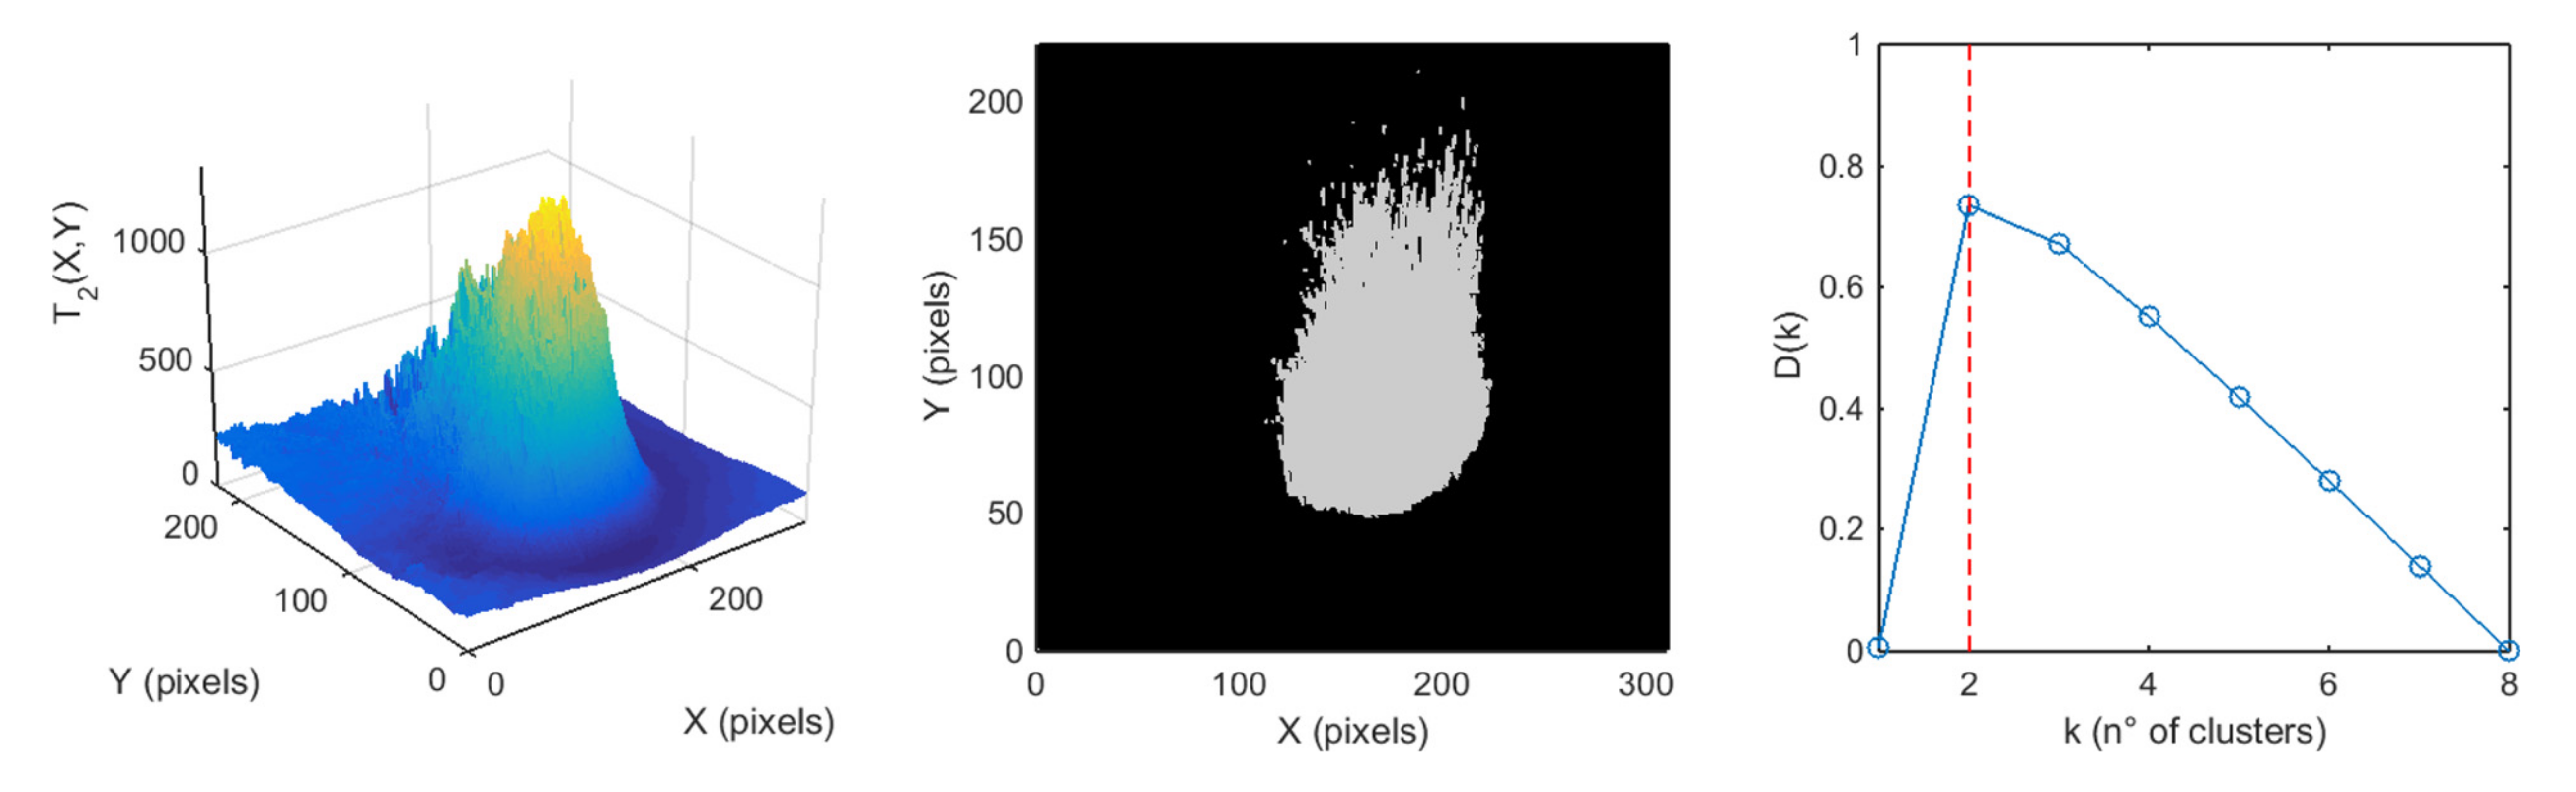
\includegraphics[width = 0.75 \textwidth]{Images/2kPCA.png}}
    \qquad
    \subfloat[\label{fig:3kpca}]{
    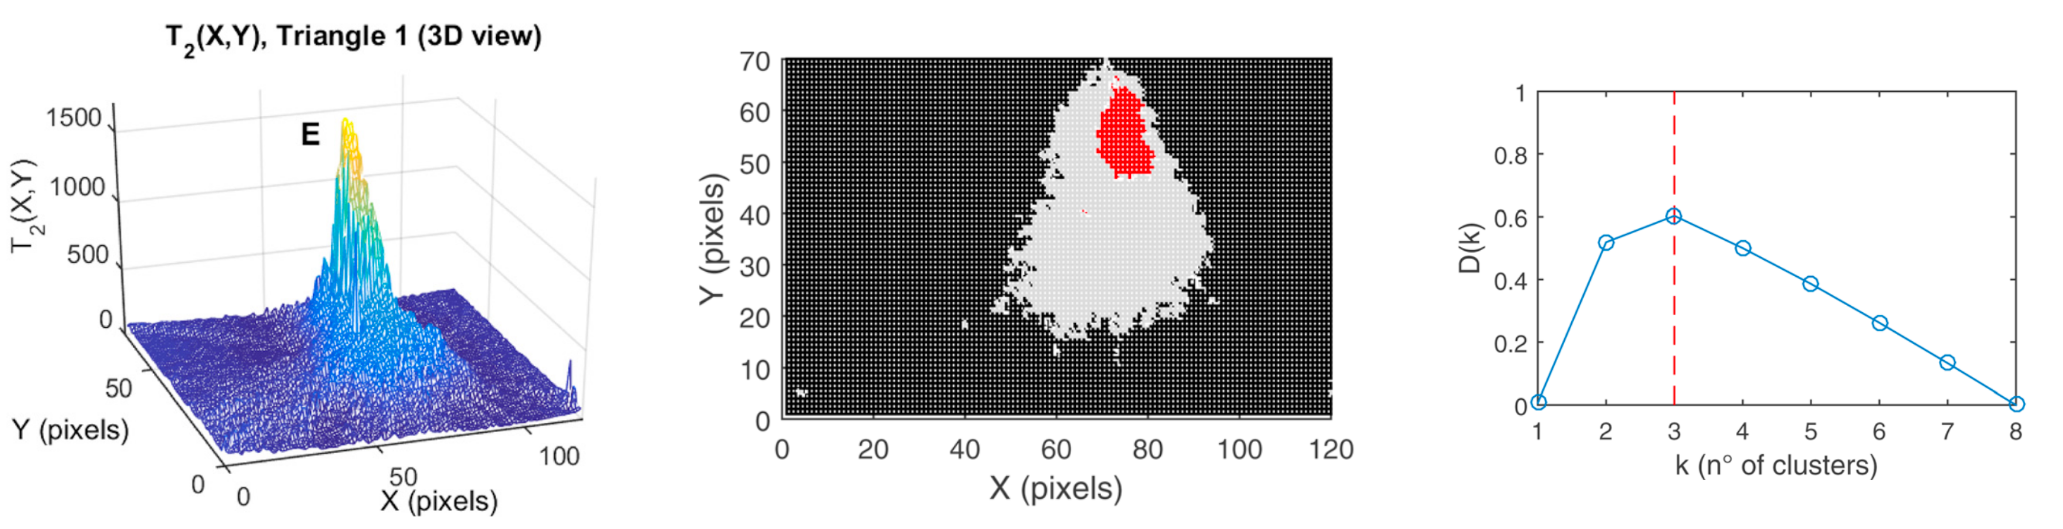
\includegraphics[width = 0.75 \textwidth]{Images/3kPCA.png}}
    \caption[T-PCA approach for HS detection.]{Spatial distribution of $T^2(X,Y)$ (left), clusters identified using the kmeans approach (centre) and corresponding $D(k)$ statistics (right) for an in control layer (a) and for an OCC (b) \cite{grasso_-process_2017}.}
\end{figure}
In the paper mentioned above, the $T_l^2$ is a spatial indicator through the mapping $T_l^2 \in \mathbb{R}_{+}^p \rightarrow T^2(X, Y) \in \mathbb{R}_{+}^{M \times N}$. Hence, it can be represented in the same domain of original images, $T^2(X, Y)$, where $X$ and $Y$ denote the image pixel location. The spatial distribution of $T^2(X, Y)$ is, therefore, suitable to synthesize the information content of a video, represented in terms of a three-dimensional array, into a spatially distributed descriptor. After obtaining the distribution of the summary index over the image domain, we can move on to the automated defect detection technique based on k-means clustering. When applied to images or surface data, the K-means algorithm segments $k$ distinct areas characterized by a maximum within similarity. In this case, the algorithm is not applied directly to the pixels but to the values of the descriptor $T^2(X, Y)$, and each pixel is assigned to the closest centroid in terms of the Euclidean distance between the values of $T^2(X, Y)$. In the defect-free case, we expect to find two clusters in the image, the first corresponding to the background (loose powder) and the second to the trace left by the laser or the spatters emitted during fusion (foreground). If defects are present, we expect a third area to be identified. The proposed method consists of clustering the spatial distribution of $T^2$ with the aim of finding, according to a data-driven approach, the optimal number of clusters $k$. In the case where the optimal number of clusters $k>2$, we can raise an alarm. The most commonly used method for finding the optimal number of clusters is to identify a knee point in the graph of the sum of squared within-distances (SSWs) as a function of $k$. The SSWs are computed as 
\begin{equation}
\begin{aligned}
\operatorname{SSW}(k) & =(1 / k) \sum_{k=1}^K \sum_{i \in c_k}\left\|T_i^2(X, Y)_{c_k}-\overline{T^2}(X, Y)_{c_k}\right\| \\
k & =1,2, \ldots, K
\end{aligned}
\end{equation}
Computationally, to find the elbow of the graph, one calculates the distance $D(k)$ between SSW(k) and the straight line connecting the two extreme points of the graph, SSW(1) and SSW(K), and then selects the estimated optimal $\hat{k}$ corresponding to the maximum distance. Formally
\begin{equation}
\hat{k}=\operatorname{argmax}_k D(k)
\end{equation}
The authors also proposed a method to be able to use T-PCA within-layers. The method described so far has a drawback that could be a bottleneck for it to be applied in real-time. Indeed, we have to wait until the scanning phase is finished since we need all $J$ frames of the image stream. However, adopting a batch processing approach can speed up the computation. This method consists of starting to process frames from the same batch before they are collected. Let $\mathcal{U}_1 \in$ $\mathbb{R}^{J^{\prime} \times M \times N}$ be a first batch of $J^{\prime}$ frames such that $1<J^{\prime} \leq J$ and let $\mathbf{X}_1$ be its unfolded version. We can repeat these steps until the level scanning is complete. By analyzing the variance-covariance structure of these first $J^{\prime}$, we can check whether an alarm has occurred from frame $j=1$ up to frame $J^{\prime}$. The model can be updated when a new batch of frames $J^{\prime}$ is available, such that $2 J^{\prime} \leq J$. The spatial descriptor can also be updated, leading to a new spatial distribution, $T_2^2(X, Y)$, and an update of the clustering analysis. The method for automated defect detection allows alarms to be identified even during the update phase. In Fig. \ref{fig:2kpca}, we can see an example of a frame in control segmented into two clusters (in grey the spatter and the laser and in black the background), while in Fig. \ref{fig:3kpca} an example of a frame segmented into three areas (in red is marked the identified anomaly).

% SPATIALLY WEIGHTED
\paragraph{Spatially weighted PCA.} In \citeauthor{colosimo_spatially_2018} (2018), the authors proposed a method to detect HS by using a spatially weighted T-PCA (ST-PCA). We can consider this approach as an extension of the PCA approach described above. Indeed, if the T-PCA allows us to consider temporal dependence, the ST-PCA also allows us to consider spatial dependence. This is made possible by defining a matrix of spatial weights $\mathbf{W}$ of size $p\times p$ where $p = M \times N$. The $(k,h)$-th element quantifies the spatial dependency between the $k$-th and $h$-th pixels (the higher the value, the higher the dependency). To calculate the $\mathbf{W}$ matrix, three different approaches were proposed in the paper, hereafter called $W_1$, $W_2$ and $W_3$.
\begin{equation}
    \begin{gathered}
\mathrm{W}_1:\left\{w_{i, j}=\frac{1}{d_{i, j}^2}\right\} \\[0.3cm]
\mathrm{W}_2:\left\{w_{i, j}=1 \text { if } d_{i, j} \leq r, w_{i, j}=0 \text { otherwise }\right\} \\[0.3cm]
\mathrm{W}_3:\left\{w_{i, j}=\left(1-d_{i, j} / r^2\right)^2 \text { if } d_{i, j} \leq r, w_{i, j}=0 \text { otherwise }\right\}
\end{gathered}
\end{equation}
where $d_{i, j}$ is the Euclidean distance between the $i$-th \& $j$-th pixels of the image, and $r$ is a reference distance threshold. This threshold is used in calculating the $W_2$ and $W_3$ weights: these methods assign a weight equal to zero to all points with a distance greater than $r$. In the case of the above mentioned study, $r=5$. Then, the spatial weights matrix is used to penalize the spectral decomposition of the sample covariance matrix. Indeed, in the case of ST-PCA the variance-covariance matrix is defined as
\begin{equation}
    \mathbf{S}=  \frac{1}{p-1}(\mathbf{X}-\mathbbm{1} \overline{\mathbf{x}})^T \mathbf{W}(\mathbf{X}-\mathbbm{1} \overline{\mathbf{x}})
\end{equation}
where $\mathbf{X} \in \mathbb{R}^{\boldsymbol{p} \times \boldsymbol{J}}$ is the data matrix of the T-mode PCA formulation, $\overline{\mathbf{x}} \in \mathbb{R}^{1 \times J}$ is the sample mean vector and $\mathbbm{1}$ is a $p \times 1$ vector of ones.
\begin{figure}
    \centering
    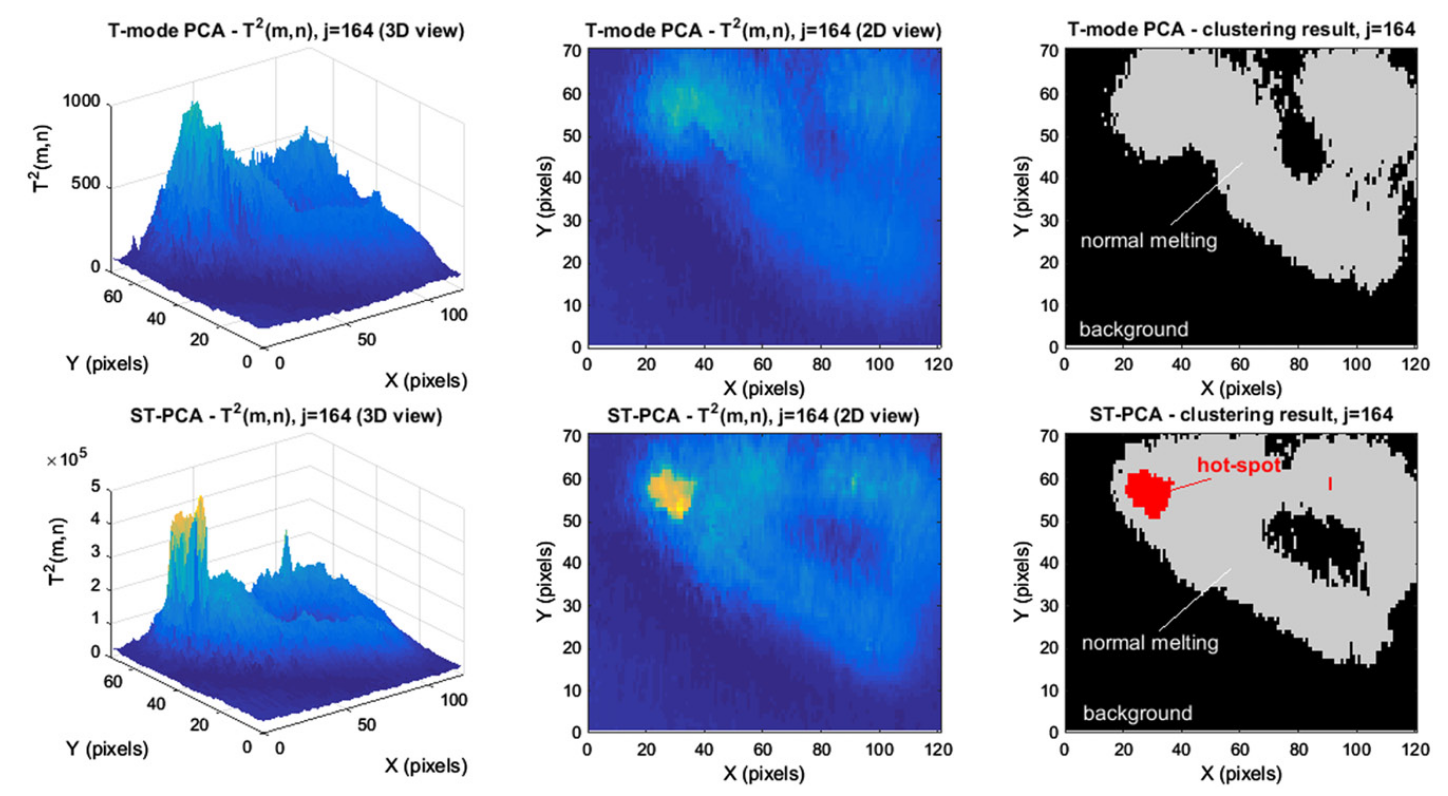
\includegraphics[width = 0.8 \textwidth]{Images/ST-PCA vs T-PCA.png}
    \caption[ST-PCA compared to T-PCA]{Results of T-mode (upper panel) and ST-PCA (lower-panel) based methods with recursive updating \cite{colosimo_spatially_2018}.}
    \label{fig:tpcavsstpca}
\end{figure}
As in \citeauthor{grasso_-process_2017} (2017), the authors used the Hotelling's distance $T^2\in\mathbb{R}^{M\times N}$ and the automated rule for the identification of HS based on K-means clustering. Furthermore, they proposed two different methods to perform iterative updating of the ST-PCA so that it can also be used with non-stationary processes: the recursive updating approach (i) and the moving window updating approach (ii). The basic idea using approach (i) is to augment the data matrix by adding each new observed frame unless an OOC state is identified. Thus, given the fact that $\boldsymbol{X}_{1: p, 1: j}$ is the data matrix that includes $j$ frames when a new frame becomes available, it is augmented to $\mathbf{X}_{1: p, 1: j+1}$. Then, we can compute the new ST-PCA model. If the pattern of the resulting synthetic statistic, $T^2(m, n)$, is judged in control, the procedure is repeated for the following frame. Otherwise, an alarm is signaled. Approach (ii), however, involves keeping the temporal dimension $L$ of the data matrix fixed. Thus, once the first $L$ frames have been acquired, the oldest frame is discarded each time a new one is acquired. If the pattern of the resulting synthetic statistic, $T^2(m, n)$, is judged in control, the procedure is repeated for the following frame. Otherwise, an alarm is signaled. We can use this approach by applying it to individual frames or batches of frames. The last approach is a great way to make the algorithm more computationally efficient. However, the larger the batch size, the longer the delay with which an alarm is detected. The authors compared this new method with the method used in \citeauthor{grasso_-process_2017} (2017). From Fig. \ref{fig:tpcavsstpca}, we can see how this new one identifies areas previously classified as in control.
\begin{figure}
    \centering
    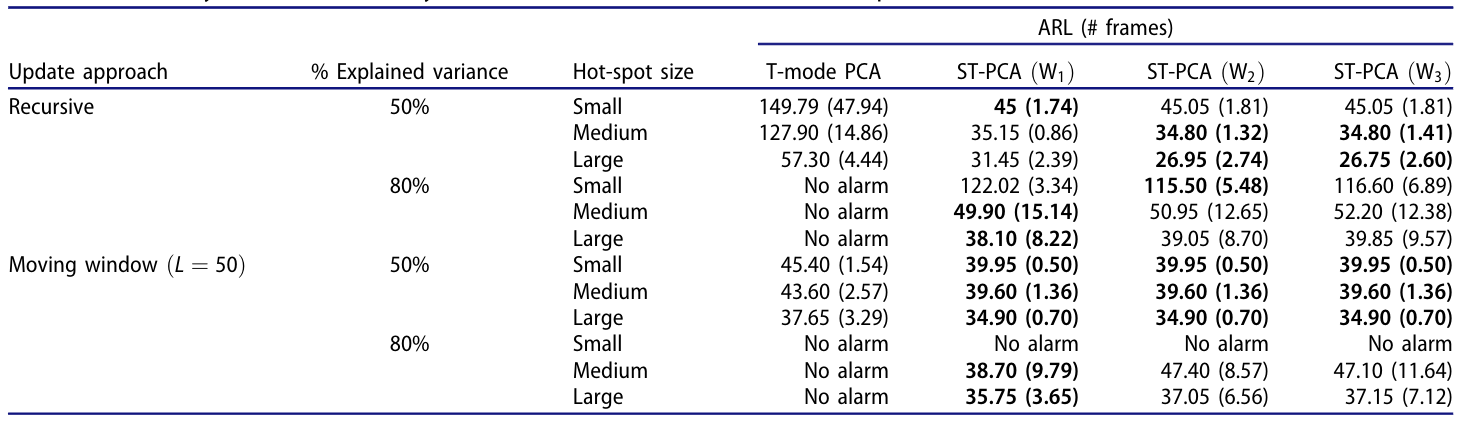
\includegraphics[width = \textwidth]{Images/firstcomp.png}
    \caption[ST-PCA simulation analysis results.]{Summary of simulation analysis results for three levels of simulated hot-spot size of $n=9$ (small), $n=20$ (medium) and $n=45$ (large) \cite{colosimo_spatially_2018}.}
    \label{fig:primocomparison}
\end{figure}
In Fig. \ref{fig:primocomparison}, we can see the different performances of the two proposed approaches as the size of the simulated defect, the method used to calculate the weights $w_{i, j}$, and the percentage of explained variance by the retained PCs vary. The simulation study was done by artificially altering the intensity of selected cross-shaped pixels of different sizes. From Fig. \ref{fig:primocomparison}, we can see how the ST-PCA outperforms the T-PCA in terms of ARL in all scenarios, sometimes even identifying defects that the previously proposed approach had not been able to detect. Recall that the ARL is the average run length, i.e., the number of frames before the defect is detected. Furthermore, we can appreciate how, in general, the approach for updating the ST-PCA based on the moving window of $L=50$ frames tends to outperform the recursive approach. This happens because the model's "memory" in terms of frames in the case of the moving window is shorter than the recursive updating approach. Therefore, it is more sensitive to OOC observations. Finally, we can see that the choice of methodology for calculating the weights $w_{i,j}$ is almost irrelevant in the case of the moving window. At the same time, the $W_2$ and $W_3$ methods are dominant with the recursive updating approach.

% REGRESSION
\paragraph{Spatio-temporal regression.} In \citeauthor{yan_real-time_2021} (2021), the authors proposed a penalized non-parametric regression model and recursive estimation algorithm so that the spatial and temporal correlation of defects could be taken into account. It is a highly-scalable spatio-temporal decomposition methodology to detect structured anomalies in real-time. The method is based on two common assumptions regarding HS events: natural events (in-control), such as the emission of plumes and spatters, are random in both the space and time domains, while HS events are localized in areas and consistent in space and time. Let $x_{s,t}$ be the pixel intensity at location $s$ and time $t$ we can then decompose it into the background $\mu_{s, t}$, a natural foreground event $u_{s, t}$, an anomaly foreground event $a_{s, t}$, and noise $e_{s, t}$ as
\begin{equation}
\label{eq:decreg}
x_{s, t}=\mu_{s, t}+u_{s, t}+a_{s, t}+e_{s, t}, \quad s=1, \ldots, S, \quad t=1, \ldots, T \text {, }
\end{equation}
where we assume that the background $\mu_{s, t}$ is known and $e_{s, t}$ follows an i.i.d normal distribution. However, $u_{s, t}$ and $a_{s, t}$ are unknown and should be estimated. We can model the anomaly as a first-order model with parameter $a_{s,t}=\theta_sx_{s,t-1}$. Substituting the relation just defined into Equation \ref{eq:decreg}, we obtain that
\begin{equation}
x_{s, t}=\theta_s x_{s, t-1}+\mu_{s, t}+u_{s, t}+e_{s, t}
\end{equation}
where $u_{s, t}$ and  $\theta_s$ are the parameters to be estimated. 
This parametric model was chosen after analyzing data from an observed HS phenomenon. As mentioned, in the presence of HS, the pixels show a higher and sustained intensity over time, characterized by a slow cooling phase. If we model the anomaly with an autoregressive model, we can capture the time dependence of the pixel with sustained intensity. Indeed, the cooling rate in normal conditions is so fast that the pixel intensity drops down to the background level from one frame to another, presenting as individual spikes. In the presence of HS, then, the parameter will be able to capture temporal autocorrelation, i.e., $\Theta_s \neq 0$ 
For the algorithm to be applicable in real-time, the estimation of these parameters must be data-driven. We can then estimate them with the penalized likelihood loss function:
\begin{equation}
\label{eq:likelihood}
\begin{aligned}
l_t\left(\boldsymbol{\theta},\left\{u_{s, t}\right\}_{s=1, \ldots, S}\right) & \\
= & \left(\sum_{s, t}\left\|x_{s, t}-\mu_{s, t}-u_{s, t}-\theta_s x_{s, t-1}\right\|^2+\gamma_1\left\|u_{s, t}\right\|_1\right)+ \\
& \quad+\gamma_2\|\boldsymbol{\theta}\|_1+\gamma_3\|\boldsymbol{\theta}\|_{T V}+\lambda_0\|\boldsymbol{\theta}\|^2
\end{aligned}
\end{equation}
where $\sum_{s, t}\left\|x_{s, t}-\mu_{s, t}-u_{s, t}-\theta_s x_{s, t-1}\right\|^2$ is the sum of squared errors and $\bm{\theta}=\left[\theta_1, \ldots, \theta_S\right]^{\prime}$. The penalties $\left\|u_{s, t}\right\|_1$ and $\|\boldsymbol{\theta}\|_1$ lead to the sparse estimation of natural and anomaly events, respectively. In order to be able to capture the spatial dependence as well, in Equation \ref{eq:likelihood} the term $||boldsymbol{\theta}||_{T V}=||\boldsymbol{D} \boldsymbol{\theta}\|_1$ was added, where $\boldsymbol{D}$ is defined as
\begin{equation*}
    \boldsymbol{D}=\left[\begin{array}{cccc}
1 & -1 & & \\
& \ddots & \ddots & \\
& & 1 & -1
\end{array}\right]
\end{equation*}
Finally, also in Equation \ref{eq:likelihood}, the term $\lambda_0\|boldsymbol{\theta}|^2$ was also added to make the stoma more robust and ensure that large background areas are characterized by the same pixel intensity even in different frames. At each instant of time, it will be necessary to solve the equation
\begin{equation}
\label{eq:casinominimal}
\begin{gathered}
\min _{\left\{u_{s, t}\right\}} L\left(\boldsymbol{\theta},\left\{u_{s, t}\right\}_{s=1, \ldots,} s, t=1, \ldots, T\right) \\
=\sum_{t=1}^T \lambda^{T-t} l_t\left(\boldsymbol{\theta},\left\{u_{s, t}\right\}_{s=1, \ldots,} s\right)
\end{gathered}
\end{equation}
to identify the anomalies $\bm{\theta}$. Parameter $\lambda \in (0,1)$ is used to give more importance to the most recent data. Since Equation \ref{eq:casinominimal} must be computed recurrently, the authors proposed an algorithm called ADMM to update it computationally efficiently. As explained earlier, in the case where two pixels are not autocorrelated, we will have $\theta_s=0$, so to identify the presence of anomalous pixels, we must at each instant of time perform the following hypothesis test:
\begin{equation}
H_0: \boldsymbol{\theta}=0 \qquad H_1: \boldsymbol{\theta}=\delta \hat{\boldsymbol{\theta}}_{\gamma_2, \gamma_3}(t)
\end{equation}
We can compute the test statistics as 
\begin{equation}
\tilde{T}_{\gamma_2, \gamma_3}(t)=\frac{\left(\left(\hat{\boldsymbol{\theta}}_{\gamma_2, \gamma_3}(t)\right)^{\top} \boldsymbol{\theta}_{0,0}(t)\right)^2}{\left\|\hat{\boldsymbol{\theta}}_{\gamma_2, \gamma_3}(t)\right\|^2} 
\end{equation}
Before $\tilde{\boldsymbol{T}}_{\gamma_2, \gamma_3}$ can be used for process monitoring, the regularization $\gamma_2, \gamma_3$ should be chosen carefully, as it plays an important role in controlling the sparsity and smoothness of $\hat{\boldsymbol{\theta}}_{\gamma_2, \gamma_3}$. To make the testing statistics robust to tuning parameter selection authors proposed a modified statistic:
\begin{equation}
\tilde{T}(t)=\max _{\left(\gamma_1, \gamma_2, \gamma_3\right) \in \Gamma} \frac{\tilde{T}_{\gamma_2, \gamma_3}(t)-E\left(\tilde{T}_{\gamma_2, \gamma_3}\right)}{\sqrt{\operatorname{Var}\left(\tilde{T}_{\gamma_2, \gamma_3}\right)}}
\end{equation}
Here, the mean and variance of the $\tilde{T}_{\gamma_2, \gamma_3}$ can be estimated by the sample mean and sample variance of $\tilde{T}_{\gamma_2, \gamma_3}$ from the In-Control (IC) data. By defininig control limit $L>0$ to reach a desired ARL. If $\tilde{T}(t)>L$, the monitoring scheme would trigger an alarm. Finally, by looking at the non-zero $\boldsymbol{\theta}$ components, we can identify the area where the defect occurred. The proposed method has a computational time of about $1/30$ compared with the computational time of ST-PCA, and also has a much lower ARL, as can be seen from the table \ref{tab:last}.
\begin{table}
\small
\centering
\begin{tabular}{llllll}
\hline
\rowcolor{bluepoli!40}
Hot-spot size & \multicolumn{1}{c}{Method} & \multicolumn{1}{c}{ARL} & \multicolumn{1}{c}{Precision} & \multicolumn{1}{c}{Recall} & F-score\\
\hline \hline
\\
Small & Regression & 3.39(1.57) & 0.88(0.27) & 0.98(0.14) & 0.90(0.24) \\
$(n=4)$ & PCA & 87.66(49.48) & 0.00(0.01) & 0.30(0.43) & 0.01(0.01) \\
& ST-PCA & 73.19(1.57) & 1.00(0) & 1.00(0) & 1.00(0) \\[0.5 cm]
Medium & Regression & 2.29(0.78)& 0.97(0.11)& 0.99(0.10)& 0.98(0.10) \\
$(n=20)$& PCA& 84.81(47.61)& 0.02(0.03)& 0.31(0.43)& 0.04(0.06) \\
& ST-PCA& 65.76(2.07)& 0.83(0.01)& 0.96(0.01)& 0.89(0.01) \\[0.5 cm]
Large& Regression& 1.20(0.58)& 0.87(0.16)& 0.99(0.10)& 0.92(0.13) \\
$(n=80)$& PCA& 74.50(53.21)& 0.12(0.14)& 0.46(0.47)& 0.19(0.21) \\
& ST-PCA& 65.76(2.07)& 0.83(0.01)& 0.96(0.01)& 0.89(0.01) \\[0.5 cm]
\end{tabular}
\caption{Performances of spatio-temporal regression compared to PCA and ST-PCA. For different simulated HS sizes, are reported ARL, precision, recal and F-score, both the mean value and the standard deviation between parenthesis on multiple simulations \cite{yan_real-time_2021}.}
\label{tab:last}
\end{table}
\textcolor{red}{Manca ancora le considerazioni e le comparazione di tutti gli altri metodi. Manca anche la definizione di precision recall e F-score.}




% FUNCTIONAL DATA CLUSTERING
\paragraph{Clustering of Functional Data.} In \citeauthor{bugatti_towards_2022} (2022), the authors systematically proposed and compared different methods to identify hot spots in L-PBF processes. The dataset used is the same as in previous papers, based on ST-PCA and T-PCA conjuncted with Hotelling's distance. Please recall that Section \ref{sec:hotspot} shows an example of the complex shape. The authors systematically proposed and compared different methods to identify hot spots in L-PBF processes. In particular, all the algorithms presented in the report use the same algorithm for data extraction based on three simple steps:
\begin{enumerate}
    \item Apply a threshold to video frames to identify bright areas. The threshold was an arbitrary value of 200;
    \item Pixels within each bright region are isolated;
    \item The average brightness of the pixels in each isolated region is extracted for the subsequent $L$ frames. In this way, a time series is obtained. In the study, the authors set the parameter for the "memory" of the average to $L=10$.
\end{enumerate} the author proposed an approach based on k-means clustering of functional data, a version of the much more popular k-means clustering algorithm we saw earlier. In this case, however, we are not interested in finding simple centroids but functional centroids. Section \ref{sec:fda} will provide an in-depth description of functional data. For now, it is enough to know that functional data are data that, despite being discrete, we can assume some unknown function generated the observations. Therefore, Functional data are not stochastic variables but observations of an unknown mathematical function perturbed by a random error. Thus, let $X=\left\{x_1, x_2, \ldots, x_n\right\}$ be a given functional dataset of size $n$ to be analyzed, where $x_i$ belongs to $\mathbb{R}^m$, and $V=\left\{v_1, v_2, \ldots, v_c\right\}$ be the functional set of cluster centers, where $c$ is the number of clusters and $v_i$ belongs to $\mathbb{R}^m$. To implement this technique, although it is not common practice for this type of clustering algorithm, only two clusters were superimposed, i.e., normal and anomalous regions. The result of this algorithm is two functional data centroids, one associated with in-control and one associated with the presence of an HS. In this case, a further pre-processing step was performed to improve classification: to prevent the brightness of the pixels from starting to increase after the decay phase (perhaps due to consecutive scans), authors applied the transformation $b_{a d j}(t+1)=\min (b(t), b(t+1))$, where $b(t)$ is the brightness of the pixel at time $t$.

\begin{figure}
    \centering
    \subfloat[\label{fig:SVMHS}]{
        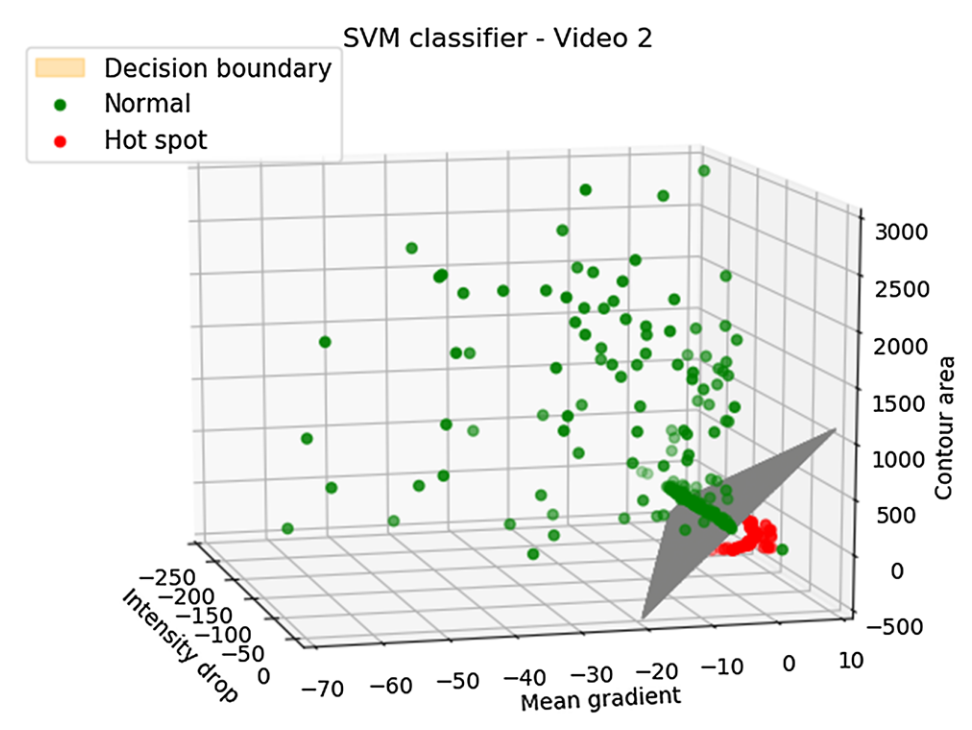
\includegraphics[width=0.4\textwidth]{Images/SVMHS.png}
    }
    \qquad
    \subfloat[\label{fig:NNHS}]{
        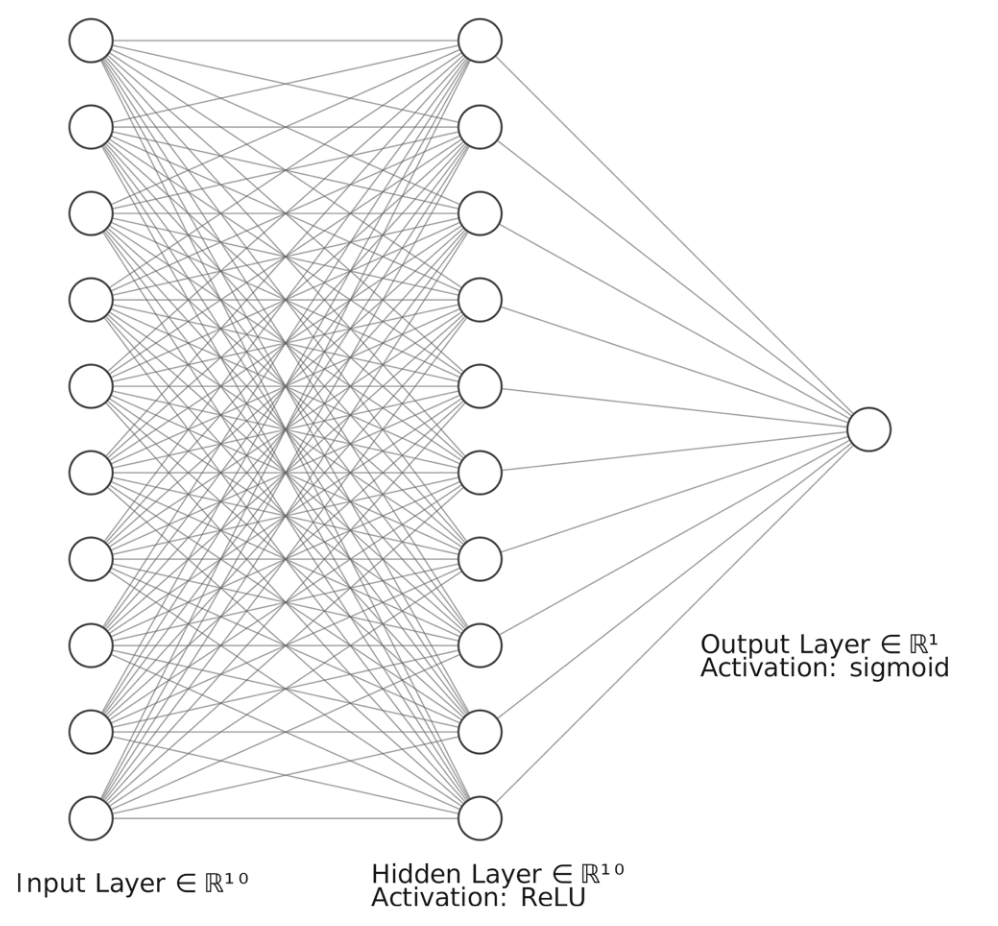
\includegraphics[width=0.35\textwidth]{Images/NNHS.png}
    }
    \caption[HS detection methods.]{Result of the K-mean functional data clustering algorithm (a), the optimal separating hyperplane in SVM (b), fully connected NN used to perform binary classification (c)\cite{bugatti_towards_2022}.}
\end{figure}


% SUPPORT VECTOR MACHINE
\paragraph{Support Vector Machine} Also, in \citeauthor{bugatti_towards_2022} (2022),
authors proposed a method to defect classification based on the use of a supervised machine learning technique called support vector machine (SVM). SVM is a machine learning technique that identifies the hyperplane between the two classes to optimize their separation. The most significant advantage of this technique is that it does not require any assumptions about the distribution of the data used as input, so it is a method that can also be applied to datasets with large dimensionality but few observations. However, this technique has a significant drawback due to its very nature: it requires labeled data for the training phase. For this reason, to avoid excessive human bias, all bright regions whose centroid lay in the acute corner area were found defective after final inspection and labeled hot-spots. Another drawback of SVM is the need to have multivariate data as input. Some SVM approaches applied to functional data have been proposed, but they are still at an 'experimental' stage, and there is no ready-to-use code routine. Hence, the authors decided to perform some feature extraction in order to be able to process multivariate data. In particular, the authors proposed to extract for each functional dataset two features:
\begin{itemize}
    \item Mean gradient
    \begin{equation}
        \overline{\Delta_1 b}=\frac{1}{L-1} \sum_{t=1}^{L-1} \Delta_1 b(t)=\frac{1}{L-1} \sum_{t=1}^{L-1}(b(t+1)-b(t))
    \end{equation}
    \item Maximum mean brightness drop between consecutive frames
\begin{equation}
    \Delta_{1, \text { max }} b=\max _{1 \leq t<L} \Delta_1 b(t)
\end{equation}
\end{itemize}
In addition, the shape and size of the bright area were also added as input data. In Fig. \ref{fig:SVMHS}, there is a graphical representation of the optimal separating hyperplane.




% DEEP LEARNING METHODs.
\paragraph{Deep learning methods.} HS detection methods using neural networks are much easier to understand and require less explanation, especially those using CNNs. Also, in \citeauthor{bugatti_towards_2022} (2022), authors proposed a method based on an NN to implement a supervised classification algorithm that finds the optimal non-linear combination of input variables to distinguish between two classes. A fully connected NN is a NN in which all neutrals are connected. In this case, since it is a binary classification problem, the output neuron will have a sigmoid activation function, and the numerical output can be seen as the probability of belonging to the success class. Like the SVM, the NN does not require any a priori assumptions about the input data distribution but requires labeled data for the training phase. For this reason, the clustered dataset using k-means clustering of functional data was used as input. The main advantage of NNs over SVM is that it does not require extracting features a priori, but NNs learn autonomously which features are significant. It will have as input the functional data extracted from the video. By doing so, we are sure to introduce no human bias and have no loss of information due to choosing the wrong feature. However, in this way, we cannot control the features extracted from the neural network. We will see in a few that by using CNNs it is possible to obtain a heat map of feature importance. For the NN-based approach to be comparable with the SVM approach, additional information about the shape and size of the identified bright regions was also given as input. The number of hidden layers and their size were treated as hyper-parameters during the choice of the network structure. Fig. \ref{fig:NNHS} presents the structure of the final NN. In \citeauthor{baumgartl_deep_2020} (2020), the authors monitored an L-PBF process with H13 material using a thermographic camera to acquire data. The camera was a PYROVIEW 640G/50 Hz/\ang{25} $\times$ \ang{19}/compact + (DIAS Infrared GmbH, Dresden, Germany), with a spectral range of \SIrange{4.8}{5.2}{\micro\metre} and an optical resolution of \numproduct{640 x 480} pixels. The acquisition frequency was set at \SI{50}{fps}. This measurement setup is a standard procedure for material analysis and process optimization. It is important to notice that this method was used for large hot spots, more similar to the so-called 'residual heat' effect that we have seen in Section \ref{sec:hotspot}. CNN has been used to classify defects from a large area characterized by prolonged overheating. The output classes used by the authors are 3: delamination, splatters, and OK (in-control). However, considering the excellent results obtained (accuracy of 97.87\% with an STD of 0.93\%), it is interesting to show the neural network structure used. In Fig. \ref{fig:cnnresidual}, there is the architecture of the final model.
\begin{figure}
    \centering
    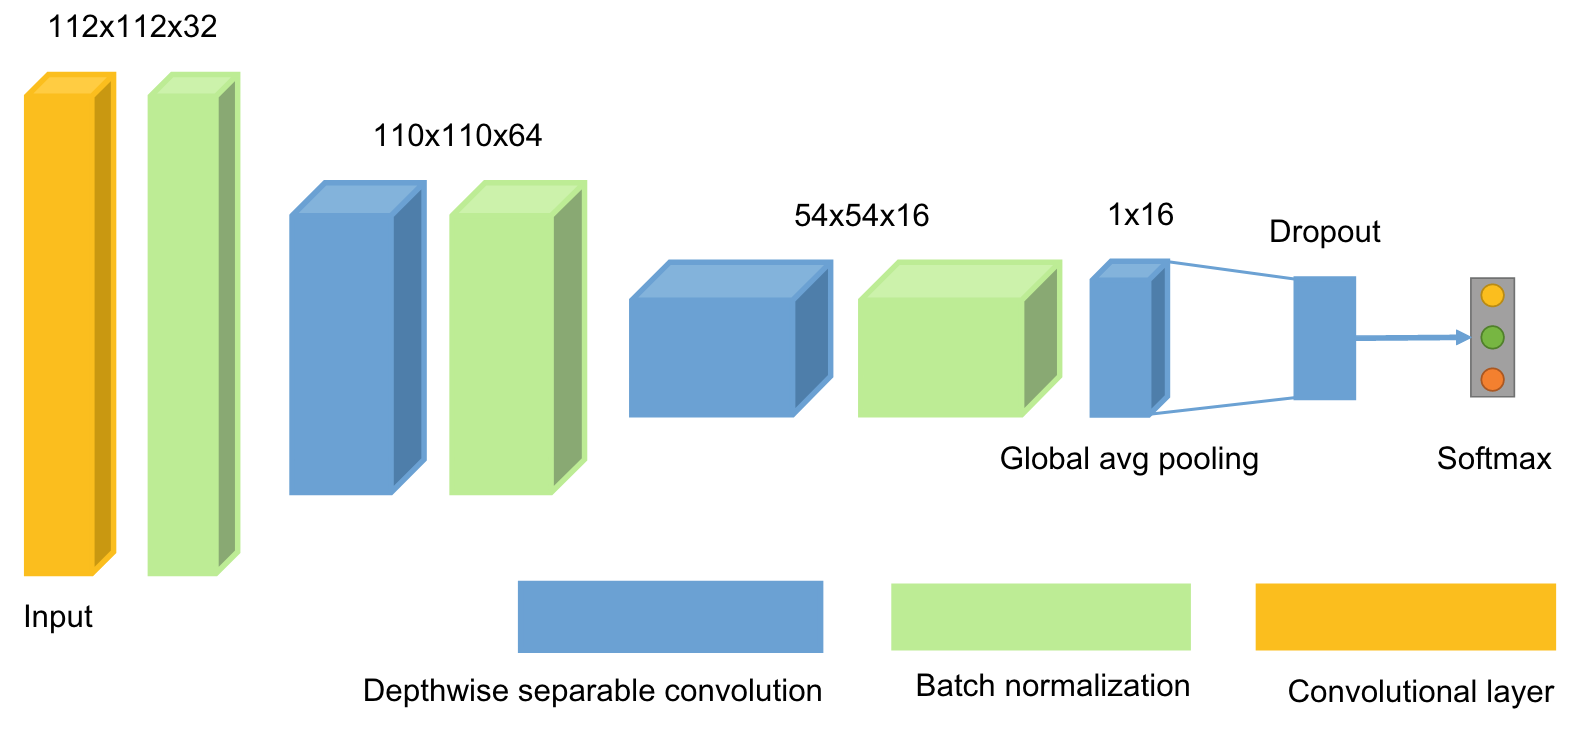
\includegraphics[scale=0.5]{Images/CNN residual heat.png}
    \caption[CNN for residual heat.]{Model architecture of the CNN for thermal data \cite{baumgartl_deep_2020}.}
    \label{fig:cnnresidual}
\end{figure}
We can also see that there are some layers we still need to discuss: the depthwise-separable convolutions. Unlike classical convolutional networks, these layers are used to learn one feature at a time. In fact, in classical CNNs, the kernel must learn spatial features and cross-channel features simultaneously. For example, with depthwise separable convolutions, we can use a 1x1 convolution layer for summarising the red-green-blue channels in a single mixed color channel and only then use a 3x3 or 5x5 convolution layer to extract the spatial features. This approach is mainly used to reduce the computational cost. Finally, with this CNN, the authors could calculate activation heatmaps. These heat maps indicate the importance of spatial features for each class. Thus, although it is a black-box model, it is somewhat interpretable. However, we cannot capture time behavior with this approach since it is based on single video frames.

% DEEP BELIEF NETWORK
\paragraph{Deep belief network.}
\begin{figure}
    \centering
    \subfloat[\label{fig:acoustic_dbn_ok}]{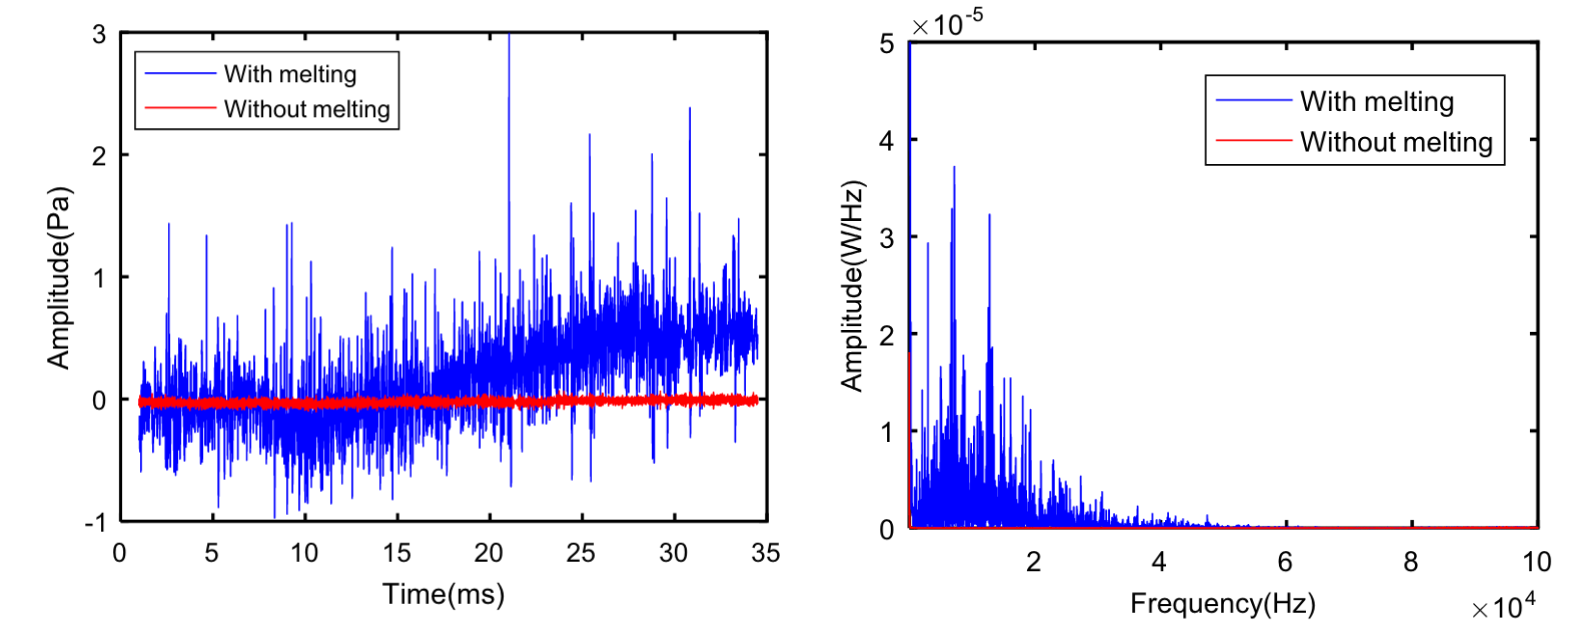
\includegraphics[width=0.65 \textwidth]{Images/dbnacoustic.png}}
    \quad
    \subfloat[\label{fig:acoustic_dbn_ooc}]{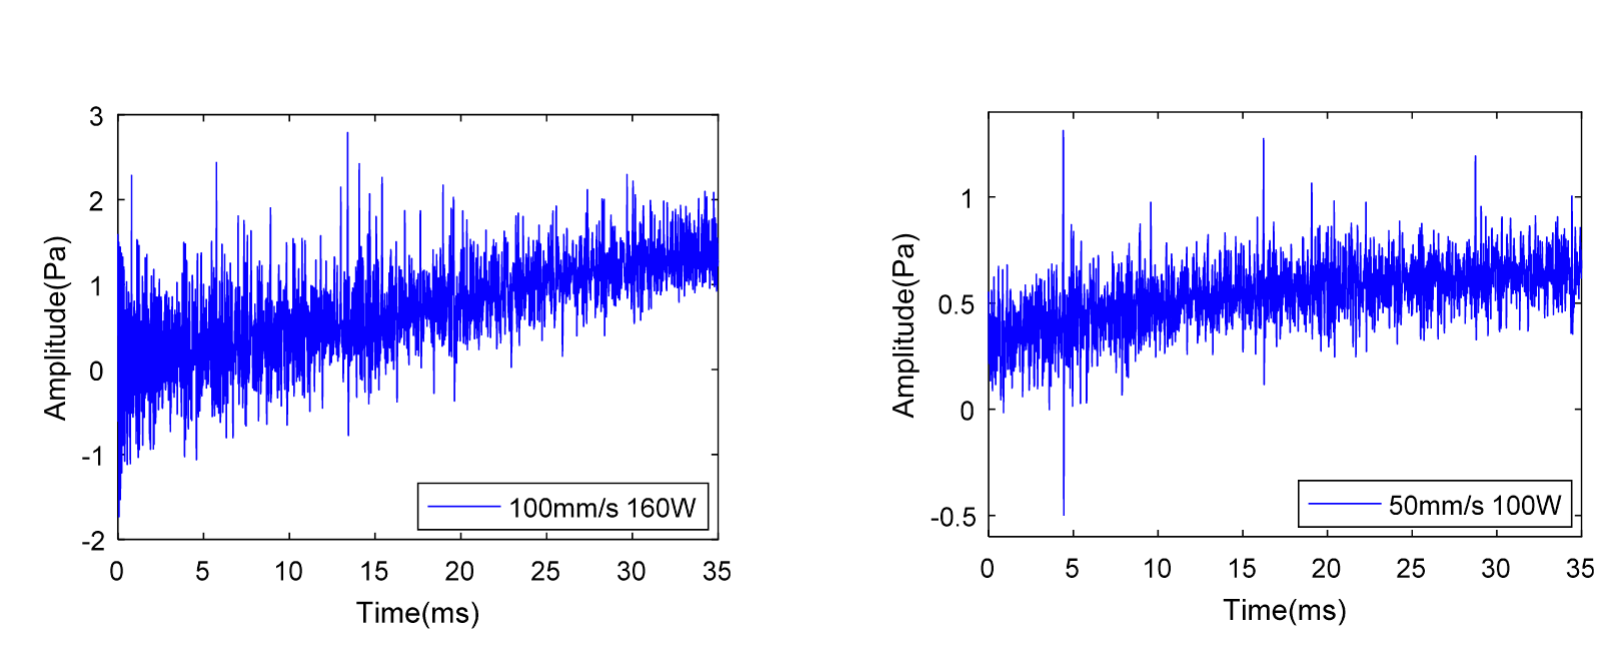
\includegraphics[width=0.65 \textwidth]{Images/defectacoustic.png}}
    \caption[Acoustics process signatures.]{Example of an acoustic signature of an in-control process (in red environmental acoustic profile) (a) and two defective acoustic signatures, one for a overheating defect (left) and one for an extreme overheating (right) (b) \cite{ye_defect_2018}.}    
\end{figure}
In \citeauthor{ye_defect_2018} (2018), authors used the acoustic signatures of the process to identify and classify five different fault categories: balling (A), slight balling (B), normal (C), slight overheating (D), and overheating (E). The air-borne acoustic signatures collected for the experiment result from plasma fluctuation during the SLS process. Underheating or overheating over metal powder by laser processing is characterized by dynamic plasma variation, leading to different acoustic profiles. In SLS, plasma is generated when highly concentrated energy irradiates the vapors that develop during printing. The air density is collected near the melting area since it is determined by the dynamics of the plasma density $N_P$. Furthermore, variations in the plasma density cause the atmospheric pressure value around the printing area to fluctuate. The acoustic intensity captured by the microphone can be calculated as
\begin{equation}
I = \frac{P^2}{f(N_P)\nu}
\end{equation}
where $P$ is the pressure, $f(N_P)$ is the air density as a function of the plasma density, and $\nu$ is the speed of sound. To acquire the acoustic signals, the authors used a microphone fixed at an angle of 30° over the platform, characterized by a frequency response from 0 Hz to 100 kHz. The sampling frequency used was 200kHz. In Fig. \ref{fig:acoustic_dbn_ok}, we can see an example of an acoustic signature of the process during the printing process (blue) and without the melting, represented both in the time domain and the frequency domain. The acoustic signature collected without melting is mainly from the machine operating and environmental noise. In Fig. \ref{fig:acoustic_dbn_ooc}, two acoustic signatures for class E and D defects can be seen. For the classification of acoustic profiles, the authors proposed using a DBN like the one in Fig. \ref{fig:dbnhsgrafica}. The training consists of five successive stages:
\begin{enumerate}
\item Train the first layer as an RBM that models the raw (frequency domain) input $\mathbf{v}=x(f)$ as its visible layer. 
\item Use that first layer to obtain a representation of the input that will be used as data for the second layer. In this case, it is the mean activations $P(\mathbf{h}^1 =1\mid\mathbf{v})$.
\item Train the second layer as an RBM, taking the transformed data as the visible layer of that RBM. 
\item Iterate 2 and 3 for the desired number of layers, each time propagating upward either samples or mean values. 
\item Fine-tune all the parameters of this deep architecture using a supervised machine learning approach for DBN.
\end{enumerate}
Overall, they achieved a classification rate of 93\%, which increased to 93.63\% after data noise reduction. It is important to note that if the data used represents the acoustic signature in the frequency domain obtained by fast Fourier transform, the classification rate increases by more than 20 percentage points. The classification rate of acoustic profiles in the time domain is about 70\%. The authors demonstrated that the proposed approach can outperform the SVM algorithm and the classical NNs. Furthermore, the advantage of this approach is that it does not require any preprocessing or feature extraction of the acquired signals, and by analyzing the connections of the RBM part, fundamental features in the classification can be understood (ed.), which could also be used in other methods.

\begin{figure}
    \centering
    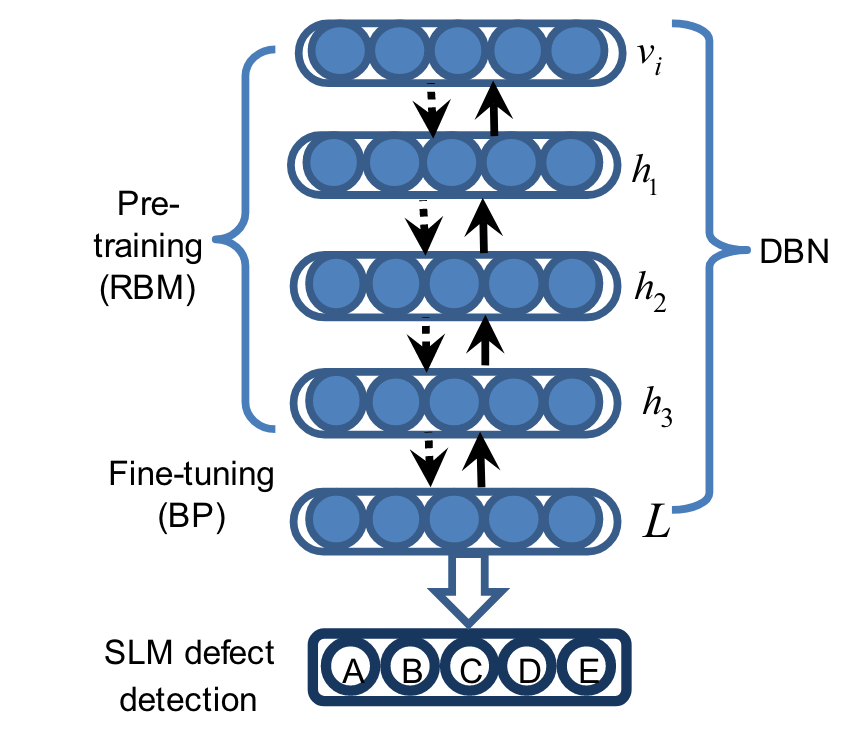
\includegraphics[scale=0.5]{Images/DBN paper.png}
    \caption[DBN used to detect HS.]{A graphical representation of the DBN used by the authors in \cite{ye_defect_2018}.}
    \label{fig:dbnhsgrafica}
\end{figure}


% Other methods
\paragraph{Other methods.} Furthermore, although it is beyond the scope of this thesis, it is worth mentioning that digital twins have been used in recent years in the scope of quality control. A digital twin is a model built using data streams to create a digital representation of a real-world asset to improve collaboration, information access, and decision-making. In other words, it combines simulation technology and real-time data. Using this technology, we can see when the printing process deviates from the simulated process and identify which process parameters to change to return to a normal condition.
% <<< End of Hot spot 